%---------------------------------------------------------------------------%
%-                                                                         -%
%-                           LaTeX Template                                -%
%-                                                                         -%
%---------------------------------------------------------------------------%
%- Copyright (C) Huangrui Mo <huangrui.mo@gmail.com> 
%- This is free software: you can redistribute it and/or modify it
%- under the terms of the GNU General Public License as published by
%- the Free Software Foundation, either version 3 of the License, or
%- (at your option) any later version.
%---------------------------------------------------------------------------%
%->> Document class declaration
%---------------------------------------------------------------------------%
\documentclass[doublesided]{Style/ucasthesis}%
%- Multiple optional arguments:
%- [<singlesided|doublesided|printcopy>]% set one or two sided eprint or print
%- [fontset=<adobe|...>]% specify font set to replace automatic detection
%- [plain]% thesis writing of international students
%- [draftversion]% show draft version information
%- [standard options for ctex book class: draft|paper size|font size|...]%
%---------------------------------------------------------------------------%
%->> Document settings
%---------------------------------------------------------------------------%
\usepackage[numbers,myhdr,list]{Style/artratex}% document settings
%- usage: \usepackage[option1,option2,...,optionN]{artratex}
%- Multiple optional arguments:
%- [bibtex|biber]% set bibliography processor and package
%- [<numbers|super|authoryear|alpha>]% set citation and reference style
%- <numbers>: textual: Jones [1]; parenthetical: [1]
%- <super>: textual: Jones superscript [1]; parenthetical: superscript [1]
%- <authoryear>: textual: Jones (1995); parenthetical: (Jones, 1995)
%- <alpha>: textual: not available; parenthetical: [Jon95]
%- [geometry]% reconfigure page layout via geometry package
%- [lscape]% provide landscape layout environment
%- [myhdr]% enable header and footer via fancyhdr package
%- [color]% provide color support via xcolor package
%- [background]% enable page background
%- [tikz]% provide complex diagrams via tikz package
%- [table]% provide complex tables via ctable package
%- [list]% provide enhanced list environments for algorithm and coding
%- [math]% enable some extra math packages
\usepackage{Style/artracom}% user defined commands
%---------------------------------------------------------------------------%
%->> Document inclusion
%---------------------------------------------------------------------------%
%\includeonly{Tex/Chap_1,...,Tex/Chap_N}% selected files compilation
%---------------------------------------------------------------------------%
%->> Document content 
%---------------------------------------------------------------------------%
\usepackage{url}
\begin{document}
%-
%-> Frontmatter: title page, abstract, content list, symbol list, preface
%-
\frontmatter% initialize the environment
%---------------------------------------------------------------------------%
%->> 封面信息及生成
%---------------------------------------------------------------------------%
%-
%-> 中文封面信息
%-
\confidential{}% 密级:只有涉密论文才填写
\schoollogo{scale=0.095}{ucas_logo}% 校徽
\title{基于深度学习的场景光照估计研究}% 论文中文题目
\author{程大川}% 论文作者
\advisor{陈彦云~研究员}% 指导教师:姓名 专业技术职务 工作单位
\advisors{中国科学院软件研究所}% 指导老师附加信息 或 第二指导老师信息
\degree{硕士}% 学位:学士、硕士、博士
\degreetype{工学}% 学位类别:理学、工学、工程、医学等
\major{计算机图形学}% 二级学科专业名称
\institute{中国科学院软件研究所}% 院系名称
\date{2019~年~6~月}% 毕业日期:夏季为6月、冬季为12月
%-
%-> 英文封面信息
%-
\TITLE{Deep Scene Illumination Estimation}% 论文英文题目
\AUTHOR{CHENG Dachuan}% 论文作者
\ADVISOR{Supervisor: Professor Chen Yanyun}% 指导教师
\DEGREE{Master}% 学位:Bachelor, Master, Doctor。封面格式将根据英文学位名称自动切换,请确保拼写准确无误
\DEGREETYPE{Engineering}% 学位类别:Philosophy, Natural Science, Engineering, Economics, Agriculture 等
\THESISTYPE{thesis}% 论文类型:thesis, dissertation
\MAJOR{Computer Graphics}% 二级学科专业名称
\INSTITUTE{Institute of Software, Chinese Academy of Sciences}% 院系名称
\DATE{June, 2019}% 毕业日期:夏季为June、冬季为December
%-
%-> 生成封面
%-
\maketitle% 生成中文封面
\MAKETITLE% 生成英文封面
%-
%-> 作者声明
%-
\makedeclaration% 生成声明页
%-
%-> 中文摘要
%-
\chapter*{摘\quad 要}\chaptermark{摘\quad 要}
\setcounter{page}{1}% 开始页码
\pagenumbering{Roman}% 页码符号


\keywords{关键词}% 中文关键词
%-
%-> 英文摘要
%-
\chapter*{Abstract}\chaptermark{Abstract}% 摘要标题


\KEYWORDS{keywords}% 英文关键词
%---------------------------------------------------------------------------%
% title page, abstract, dedication
{% content list region
\linespread{1.2}% local line space
%\intotoc{\contentsname}% add link to contents table and bookmark
\setcounter{tocdepth}{1}
\tableofcontents% contents catalog
%\intotoc{\listfigurename}% add link to contents table and bookmark
\listoffigures% figures catalog
%\intotoc{\listtablename}% add link to contents table and bookmark
\listoftables% tables catalog
}
\chapter*{缩写列表}
\chaptermark{符号列表}

% \section*{字符}
% \nomenclatureitem[\textbf{Unit}]{\textbf{Symbol}}{\textbf{Description}}
% \section*{算子}
% \nomenclatureitem{\textbf{Symbol}}{\textbf{Description}}

\section*{缩写}

\nomenclatureitem{AE}{Auto Encoder}
\nomenclatureitem{AR}{Augmented Reality}
\nomenclatureitem{BRDF}{Bidirectional Reflectance Distribution Function}
\nomenclatureitem{CNN}{Convolutional Neural Network}
\nomenclatureitem{DNN}{Deep Neural Network}
\nomenclatureitem{DSSIM}{structural Dissimilarity}
\nomenclatureitem{FOV}{Field of View}
\nomenclatureitem{HDR}{Hight Dynamic Range}
\nomenclatureitem{IBR}{Image Based Rendering}
\nomenclatureitem{LDR}{Low Dynamic Range}
\nomenclatureitem{MAE}{Men Absolute Error}
\nomenclatureitem{MSE}{Mean Squared Error}
\nomenclatureitem{PSNR}{Peak Signal to Noise Ration}
\nomenclatureitem{RELU}{Rectified Linear Unit}
\nomenclatureitem{RMSE}{Root Mean Squared Error}
\nomenclatureitem{SH}{Spherical Harmonics}
\nomenclatureitem{SHL}{Spherical Harmonic Lighting}
\nomenclatureitem{SOTA}{State of The Art}
\nomenclatureitem{SSIM}{structural Similarity}
%\nomenclatureitem{}{}% list of symbols, preface content
%-
%-> Mainmatter
%- 
\mainmatter% initialize the environment
%---------------------------------------------------------------------------%
%->> Main content
%---------------------------------------------------------------------------%
\chapter{绪论}\label{chap:introduction}

\section{选题的背景及意义}
%% 学科背景

%% 问题定义与介绍
光照估计(又称光照分布估计)是从已知的彩色图像信息中,预测、估计、恢复出整个场景的光照分布。
该问题的输入通常是若干张彩色图片,或者是一段视频,有时已知的几何或材质信息也被用来辅助估计光照。
场景的光照分布是指场景中各个方向的光照的颜色和强度。
较为常见的光照分布表示方法包括
高动态范围(High Dynamic Range,HDR)全景图、球形谐波(Spherical Harmoins,SH)函数表示、
基于物理的Sun-Sky模型表示等。
其中精度最高、使用比较广泛的是HDR全景图像,而在实时渲染领域使用较多的是光照的SH表示。 
基于物理的光照模型则多用于室外场景。

%% 研究意义、应用场景
光照估计作为计算机图形学和计算机视觉的基础问题之一,有着广泛的实际应用场景。
例如:基于图像的渲染(Image Based Rendering,IBR)、
增强现实(Augmented Reality,AR)、电影后期制作、真实感虚实交互等。
图\ref{fig:demo-problem-define}展示了光照估计的应用之一。
光照估计也与这两个学科中的许多其它问题息息相关。
例如:双向反射分布函数(BRDF)估计、场景几何重构、本征信息提取、图像增强,等等。
高质量的光照估计结果通常能够为这些问题的解决带来很大的帮助。
\begin{figure}[!htbp]
    \centering
    
\includegraphics[width=0.40\textwidth]{Img/ucas_logo.pdf}

    \bicaption[光照估计的应用]
    {光照估计的应用之一。使用单张图片估计场景的光照,并利用估计的光照渲染一个新的物体合成到图像中。
    可以看出使用估计光照渲染后的3D物体,与场景中的已有物体在视觉上较为一致。}
    {3D rendering under the predicted illumination.
    visual effect of the 3D rendering is in line with the original image.}
    
    \label{fig:demo-problem-define}
\end{figure} 

%% 难点
从有限的图像信息估计出整个场景的光照分布是一个复杂的问题。
首先,图像的视野范围比较有限,
例如一张视场角(FOV)为60°的照片所拍摄到的区域,在其对应的全景图中占比不足6\%。
此外,一幅图片是光照分布、场景几何结构、物体材质、摄相机参数等多个单位之间的复杂交互结果
(公式~\ref{eq:complex-interaction-result})。
\begin{equation} \centering \label{eq:complex-interaction-result}
Image = ComplexInteraction(Light, Geometry, Material, Camera)\end{equation}
通过公式\ref{eq:complex-interaction-result}可以看出,
在其它三个信息未知的情况下,从图像(Image)反推出光照(Light)是一个严重的不适定(ill-posed)问题。
不仅如此,在不同的条件下拍摄的彩色图像可能存在很多误差。
例如图像中的过曝光/欠曝光区域、相机畸变、不正确的白平衡等。
这些都会对光照估计造成一定程度的干扰,增加光照估计的难度。

%% 传统方法 + 局限性
研究者们在光照估计问题上开展了一系列的研究。Debevec\cite{debevec1998rendering}
首次提出可以通过拍摄不同曝光下的镜面球体,来获取一张高动态范围的全景图片。
\todo{Related limited methods.} 
不难看出,这些方法或依赖特殊的探针、或依赖特殊的拍摄设备、或依赖额外的辅助信息与模型假设。
均具有一定的局限性。

%% 深度学习方法 + 局限性
近年来,深度学习在多种计算机视觉问题上大放异彩,用于分割、检测、标识、分类的神经网络层出不穷。
一些研究者尝试将深度学习应用在光照估计问题当中。
\todo{Related learning based methods.}
不过,目前已有的深度学习方法也有一定的局限性。
训练一个鲁棒的神经网络往往需要大量的数据,而目前用于光照估计问题的数据集比较有限,主要包括:
大规模的低动态范围全景数据集(SUN360\todo{CITE}等)和
中小规模特定场景的高动态范围全景数据集(Laval Indoor等\todo{CITE})。
这些数据集在规模和质量上很难同时到达训练深度神经网络的要求。

%% 研究目标和研究方法, 在前人工作的基础上,对网络、loss、优化,数据 展开研究
在这样的背景下,本文在光照估计的两个方向开展研究。
其一是构建一个具有一定规模和质量光照估计的数据集。
这样的数据集不仅能被用来训练更加鲁棒的光照估计网络,也可以被应用到其它多种相关的深度学习问题当中。
其二是在已有数据集和本文构建的数据集基础上,深入探索基于深度学习的光照估计方法,
对其中的网络结构,网络参数,损失函数,光照表示等多个模块进行细致的对比和研究。

\section{国内外研究现状}
\subsection{光照的表示}
光照的表示对光照估计问题至关重要。
场景的光照分布有着多种多样的表示方法。其中
高动态范围(High Dynamic Range,简称HDR)全景图是一种被广泛使用而且精度较高的光照表示方式。
与普通的8位三通道图像不同,HDR图像的颜色值范围可以从0取到非常大。
这意味着HDR图像可以更细致地表示每个像素位置的真实亮度值。
因此无论是HDR全景图表示的光照,还是使用其渲染的物体,都能更接近真实值。
Reinhard等人在\textit{High Dynamic Range Imaging}\cite{reinhard2005high}中对HDR图像进行了详细的介绍。

%%HDR全景图表示的光照在图像渲染、估计光照等问题中往往比较“繁琐”。
研究者们也提出了一些小巧、高效的光照近似模型,代价是牺牲一部分精度。
Ramamoorthi和Hanrahan\cite{ramamoorthi2001efficient}提出使用球形谐波函数来表示场景的光照。
这种方法表示的光照,不仅参数规模较小,而且其在渲染物体时非常高效。
他在文章中指出,该模型仅使用9个系数时,在漫反射物体上渲染结果的平均误差也不超过1\%。
不过由于球形谐波函数本身的特性,这种方式不能很好的保留光照分布的高频细节。
尽管如此,它的简洁和高效使得它成为实时渲染中的重要方式之一\cite{green2003spherical,sloan2008stupid}。
许多光照估计方法中采用了这种模型来表示场景的光照分布。
图\ref{fig:lighting-representation}展示了不同的几种光照表示示例。
\begin{figure}[!htbp]
    \centering
    
\includegraphics[width=0.40\textwidth]{Img/ucas_logo.pdf}

    \bicaption
    {几种不同的光照表示模型对比}
    {Comparison of different representations of illumination}
    
    \label{fig:lighting-representation}
\end{figure}

在室外场景中,光线的主要来源是太阳光、光在空气中的散射折射、以及光在地面的反射。
因此基于物理的光照表示模型更加适合表示室外场景。
Perez等人\cite{perez1993all}提出一个参数化的物理模型来表示天空中的发光度(Luminance)分布。
之后的许多工作
~\cite{nishita1996display, sirai1993display, preetham1999practical,raab2008unbiased}
考虑了空气散射和折射、大气浑浊度的影响,将该模型扩展为多种不同类型颜色模型。
Hosek和Wilkie\cite{hosek2012analytic, hovsekhovsek2013adding}基于这些工作,
考虑并加入了多种因素,整理出一个可调节太阳位置、大气浑浊度、地面反照率的物理参数模型。
这类模型的参数量较小,精度也很可观,因此成为室外场景光照估计问题中常用的光照表示方法。

光照分布也有很多其它的表示方式。
Ng等人\cite{ng2003all}提出使用小波函数来近似光照分布。
LeGendre等人\cite{legendre2016practical}提出了一个实用的框架,
能够使用LED灯台精确地重构出各个方向的场景光照。
近期Weber\cite{weber2018learning}结合深度学习,
使用自编码器(auto-encoder)对光照分布进行建模,为光照估计问题提供了新的思路。

\subsection{使用光探测物估计光照} 
光照估计是一个复杂的问题,研究者们常常采用多种方法的组合来解决这个问题。
使用光探测物(light probe)来估计光照就是这些方法之一。
常见的光照探测物包括:
镜面球体,漫反射球体,镜面反射/漫反射混合球体,人眼,人脸等等。
Debevec\cite{debevec1998rendering}建立了一个基于光照模型的虚拟物体插入系统。
其中所涉及光照的就是使用镜面反射球体作为光探测物来估计的。
该工作首次提出可以通过拍摄不同曝光下的镜面球体,来获取一张高动态范围的全景图片。
在之后的工作中,Reinhard等人\cite{reinhard2005high}和Debevec等人\cite{debevec2012single}指出,
使用一个漫反射球体,或者漫反射与镜面反射表面混合的球体,也可以达到同样的效果。 
值得一提的是,Debevec在其工作\cite{debevec1998rendering}中,
将远距离场景、近距离场景、以及待插入的虚拟物体分离开,
并假设插入的虚拟物体并不会造成远距离场景的变化。
之后的虚拟物体插入、增强现实等工作都遵从了这个假设。

上述的光探测物大多是已知物体几何和表面材质、且预先放置在场景中的规则物体。
还有一些特殊的“物体”也可以作为光探测物。
例如人的眼球,人脸,人手等常出现照片中的元素。
Tsumra等人\cite{tsumura2003estimating}在假设人眼是规则球体的前提下,
利用眼球上光线的反射,估计场景的光照。
Nishino和Nayar\cite{nishino2004eyes}分析了眼球的大致结构,并利用包含眼球的照片估计场景的光照分布。
不过该方法需要分辨率和清晰度较高的相机,而且其文中也指出该方法没有考虑瞳孔颜色、虹膜颜色等因素。
而这些因素都会对光照估计产生较大影响。人脸作为照片中经常出现的物体,也经常被用作光探测物。
Wen等人\cite{wen2003face}通过一张人脸照片,估计出光照的SH表示进而对人脸实现重照(relight)
Wang等人\cite{wang2007face}提出来一种基于马尔科夫随机场的能量最小化框架,意图从正脸照片中恢复出人脸的形状、反照率和光照。   
在之后的工作中Shim\cite{shim2012faces}、Knorr等人\cite{knorr2014real}、
Shahlaei和Blanz\cite{shahlaei2015realistic}探索了如何从人脸照片中估计较为精确的光照。
Yao等人\cite{yao2013hand}使用普通相机和深度相机下的人体手部图像,
通过人手的亮度和法线,估计出由若干个球形谐波系数近似的低频光照。

可以看出,这类估计光照的方法都需要一个已知其类型、几何、材质的光探测物存在于场景内。
无论是规则的球体,还是人的各个部位,它们都需要照片中包含指定的物体和元素。
而在大多数的光照估计问题中,很难保证这些标志物或探测物一定存在,这无疑限制了此类方法的应用。

\subsection{使用特定设备估计光照}
降低光照估计问题难度的另一个思路是使用特定的设备、装置、应用。
Pilet等人\cite{pilet2006all}使用多个不同位置的相机和一个平面标定物构建了一个3D估计系统。
通过追踪该平面标定物并计算其中的高光和阴影,估计出场景中的几何和光照。
Yoo和Lee\cite{yoo2008real}提出了一个由鱼眼镜头、
中性衰减片(Neural Density Filter,ND)和普通相机构成的光照探测系统。
他们通过鱼眼镜头获取一个半球面,使用ND片直接感知明亮区域,
并通过一系列算法实时地估计场景中的光照。
Cossairt\cite{cossairt2008light}等人使用一组透镜、光场相机、光场映射器,
构建了一个适合单光源较暗场景下的光照估计系统。
随后Imai等人\cite{imai2011estimation}使用多光谱成像设备,
探究了可变亮度阈值、色调、偏振滤镜在检测光照条件较为复杂的场景下的高光分布。
提出了适用于偏高光反射物体上的光照估计方法。
Tocci等人\cite{tocci2011versatile}构建了一个光学设备,用以获取影视级别的高动态范围视频。
Manakov等人\cite{manakov2013reconfigurable}提供了一个插件类型的相机硬件,
用以与高动态范围图像,多光谱、偏振和光场等相关的应用。
Cailian等人\cite{calian2013shading}使用一个阴影探测器,来解决实时增强现实中的光照估计问题。
K\'an和Peter\cite{kan2015interactive}通过全景图像拼接技术,建立了一个在智能相机中用于捕捉高动态范围全景图的应用。

不过,通过这些使用特殊设备或者特定应用获取场景光照的方法并不是严格意义上的光照估计。
他们其实是倾向于解决快速获取高动态范围图像或视频的工程问题。
\begin{figure}[!htbp]
    \centering
    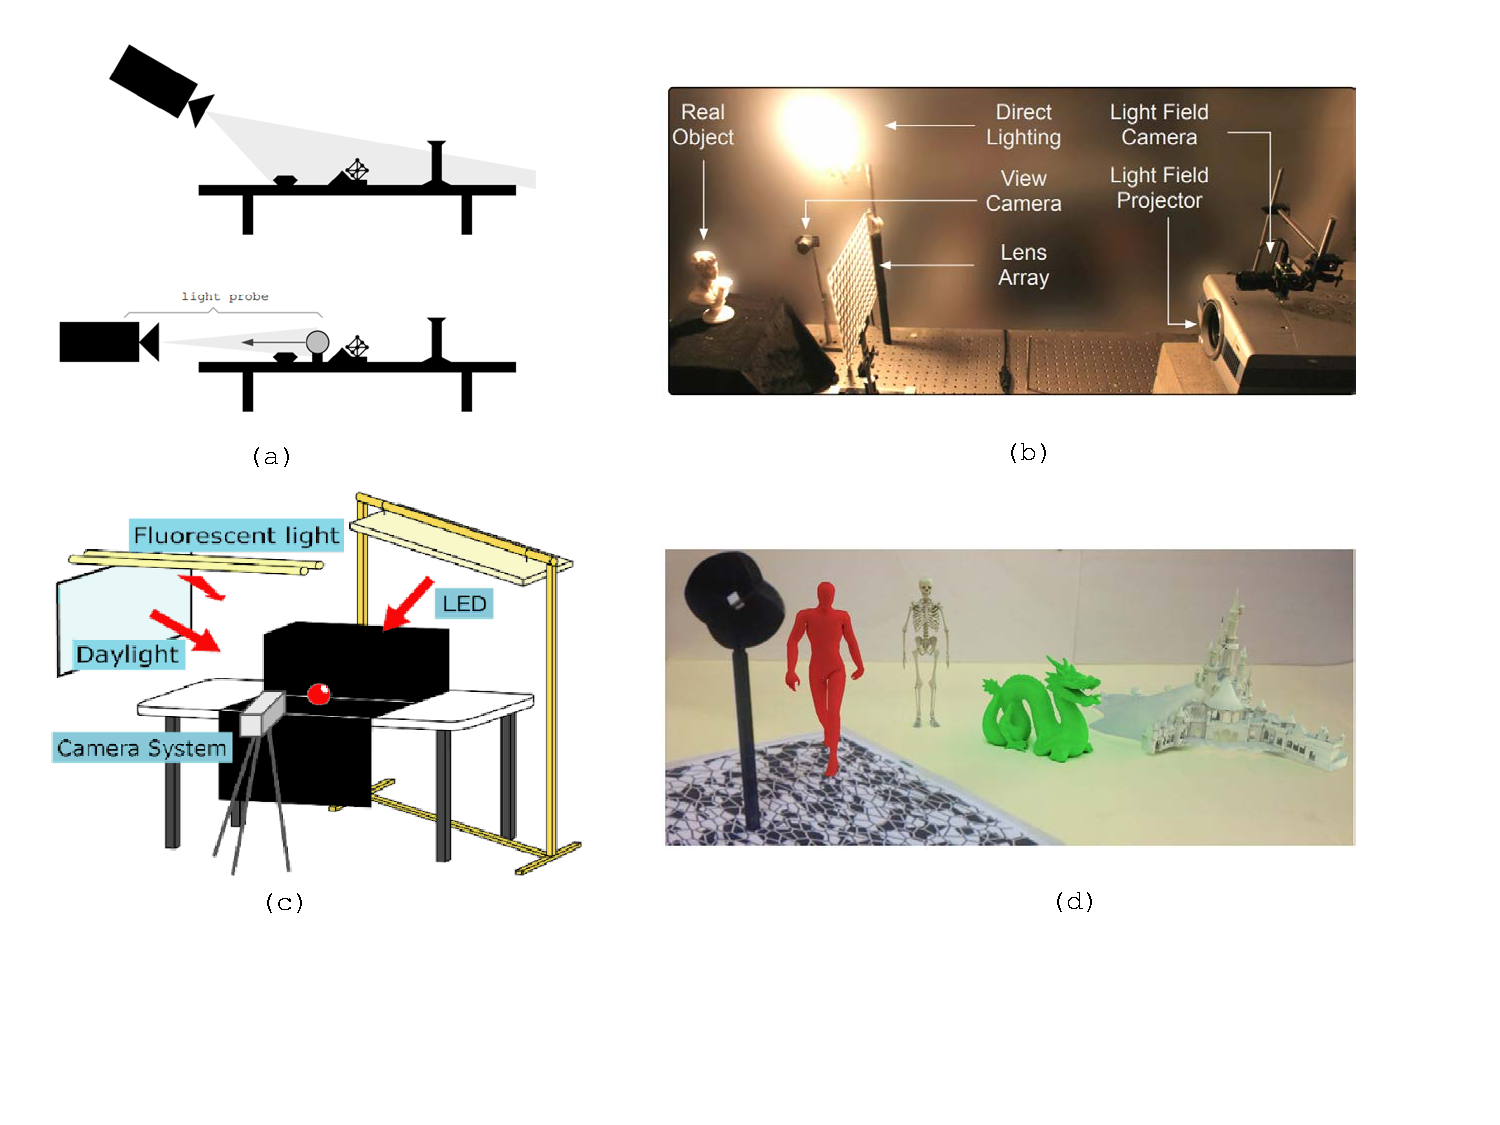
\includegraphics[width=1.0\textwidth]{Img/estimation-using-devices.pdf}

    \caption[使用特殊设备估计光照]
    {几种使用特殊设备估计场景光照的系统:(a)Debevec\cite{debevec1998rendering}通过多次拍摄获取光照的示意图;(b)Cossairt等人\cite{cossairt2008light}的复杂拍摄系统;(c)Imai等人\cite{imai2011estimation}使用的拍摄设备;(d)Cailian等人\cite{calian2013shading}用于AR光照估计的设备示意图。}
    %%{Illumination estimation system using specific devices.}
    
    \label{fig:estimation-using-devices}
\end{figure}
图\ref{fig:estimation-using-devices}
展示了上述的一些的光照估计系统的使用情景,可以看出,这种光照估计方法所需的设备通常比较复杂。
虽然在实验室环境中能够有效运行,但是这些设备的类型和数量无疑提高了这种方法的应用门槛。

\subsection{使用额外信息估计光照}
从单张图片恢复或估计出整个场景的光照分布是个复杂的问题。
大部分的光照估计方法考虑借用额外的信息来辅助估计光照。
例如,深度图像信息、场景几何形状、物体几何结构等。

深度信息对于光照估计问题有着很大的帮助。
Knecht等人\cite{knecht2012reciprocal}借助深度相机和鱼眼镜头重建场景模型并提取了光源位置。
Meilland等人\cite{meilland20133d}利用深度相机实时地创建稠密的高动态范围全景图,
并使用K-means 算法从环境贴图中提取点光源位置。 
Barron和Mailk\cite{barron2013intrinsic}提出了一种从彩色图像和深度图像中提取本征信息的方法。
他们使用具有噪声的深度图像来辅助估计场景的几何结构,并在这些信息的基础上进一步提取彩色图像中的本征信息。
Zhang等人\cite{zhang2016emptying}使用RGBD相机,
将拍摄到的室内场景建模为一个包含光源、材质和几何的没有杂物的房间模型。
并提供了对该模型进行场景编辑的方法。

在已知场景或物体几何结构的情况下估计光照的分布也是主要的研究方向之一。
例如,在形状类似桌子、平台、平板等结构的场景中,Li等人\cite{li2003multiple}的方法
可以结合图片中的阴影、明暗、高光信息估计出多个方向的光源信息。
Ramamoorthi和Hanrahan\cite{ramamoorthi2001signal}使用物体的几何结构和多个视角下的照片作为输入,
估计出照片中物体的表面材质并进一步计算所在场景的静态光照信息。
不过该方法需要多种假设——曲线表面、各向同性BRDF、没有多重反射等。
Sato等人\cite{sato2003illumination}指出通过物体遮挡关系估计场景光照的有效性。
他们通过分析给定几何的物体上的明亮区域和阴影区域,估计出较为真实的场景光照。
在给定朗伯体(Lambertian)反射的物体几何时,Wang和Samaras\cite{wang2002estimation}的方法
可以从单张图片估计出多个方向的光照信息。
Panagopoulos等人\cite{panagopoulos2011illumination}提出了一个新的框架,
来从单幅图片和粗糙的3D几何中,恢复出光照环境和估计场景中的投影阴影。
该方法描述了一个高阶马尔可夫随机场(MRF)照明模型。
该模型将低阶阴影证据与高阶先验知识相结合,用于投影阴影和照明环境的联合估计。

此外还有一些方法在已知物体类型的情况下,利用图片中物体的先验或者假设知识来帮助估计光照。
例如前文提到的Nishino和Nayar\cite{nishino2004eyes}假设人的眼球是规则的球体,
并基于此假设从人眼估计场景的光照。
类似的方法\cite{barron2015shape, lopez2010compositing, rematas2016deep}
虽然不需要预先知道精确的场景几何结构,但都要通过图像中物体的类型得到一些先验知识
假设和约束。进而分析、预测、估计、恢复出场景光照。

%% 多张图片
增加彩色图片的数量也会对光照估计有很大帮助。
Sato等人\cite{sato1999acquiring}使用两张全方位的照片构建出场景的大致几何,
然后根据不同快门速度拍摄的全方向图像序列计算场景的辐射度,并将其映射到构建的几何模型上。
这个映射到几何上的辐照度分布就可以作为光照来渲染新的3D物体。
Nishino等人\cite{nishino2001determining, nishino2005re}在已知物体的大致几何的情况下,
分别对发光体和普通物体拍摄多张图片来估计场景光照。
Yu等人\cite{yu2006sparse}则通过多视角图片来恢复出固定光照条件下的物体纹理和光照分布。
Wu等人\cite{wu2011high}建立了一个纯基于图片的形状、表面及光照估计模型。
Shan等人\cite{shan2013visual}在解决重构场景的问题时,
提出了一种从大规模的、不同光照条件下的图集中估计几何结点反照率和光照参数的方法。
受到这个方法的启发,Lalonde和Matthews\cite{lalonde2014lighting}
在同一个室外建筑物的不同图片中恢复出每幅图片对应的光照条件。

需要注意的是,以上几种增加辅助信息的方式并不是互斥的,研究者们可以选择使用多种额外信息共同辅助估计光照。
例如Marschner\cite{marschner1997inverse}在已知物体几何的前提下,
使用一组照片估计出物体表面的反射情况,进而估计出场景光照信息。
Haber等人\cite{haber2009relighting}利用一个物体在多个角度下的图片和已知几何结构估计其光照分布。
使用一种或多种额外的信息来辅助光照估计一直是解决光照估计问题的主要方法,
也是能够提升光照估计的效果的主要方式。
但是此类方法通常需要使用额外的输入设备(例如深度相机),繁琐的获取步骤(例如多次拍摄),以及一些先验知识。
而且使用的额外信息越多,所需的设备就越多,步骤就越繁琐,这难免限制了它们的应用场景。


\subsection{使用简化的光照模型估计光照}
光照估计是一个已知条件较少,求解结果复杂,涉及因素繁多的问题。
除了使用额外的设备增加输入信息规模的方法外,降低该问题难度的另一个思路是简化光照的表示。
从有限的信息中估计出复杂的场景光照分布是比较困难的,
所以许多方法尝试选取相对简单的光照近似模型表示光照,即通过牺牲一部分精度来降低待估计参数量的规模,
从而达到简化光照估计问题的目的。
其中最为常见的就是使用球形谐波(spherical harmonic)函数近似的光照模型。
该模型最早由Ramamoorthi\cite{ramamoorthi2001efficient}在2001年提出。
通过应用该模型,光照的低频部分可以使用少量的系数(通常为9-16组,约27-48个)来近似。
虽然这种表示方式对光照分布中的高频细节不太友好,但在渲染常见的漫反射物体时却有着极小的误差。
因此许多工作\cite{ramamoorthi2001signal,kemelmacher20113d,garrido2013reconstructing,
knorr2014real,li2014intrinsic,barron2015shape, rematas2016deep}
通过估计少量的SH系数来达到估计光照的目的。
与之类似,Barronhe和Malik\cite{okabe2004spherical}在光照估计问题中使用小波函数来近似场景光照,
并将其与SH表示进行了对比,指出了在表示光照时球形谐波函数相较于小波函数的优点。
早期的一些光照估计工作\cite{sato1999acquiring,  panagopoulos2011illumination, 
wang2002estimation, li2003multiple, sato2003illumination}将光照分布简化为若干个点光源的集合。
进而将光照分布估计问题转化为预测光源数量、位置和大小的问题。
预测这种类型的光照比较简单,但遗憾的是真实场景中的光照分布往往比较复杂,能够使用这种类型表示的场景并不是很多。

对于特定的场景(比如室外),基于物理模型的光照表示是一个很好的选择。
这种模型往往能够使用很小的参数量近似出精度较高的光照分布。
其中最具有代表性的是Perez\cite{perez1993all}在1993年提出的天空的发光度分布模型。
该模型经过多次补充,修改和完善\cite{nishita1996display, sirai1993display,
preetham1999practical,raab2008unbiased,hosek2012analytic, hovsekhovsek2013adding},
目前已经成为了一个包含太阳位置、大气浑浊度、地面反照率等多个具体物理意义参数的物理模型。
因此大部分室外光照估计方法\cite{lalonde2008does, lalonde2010sun, lalonde2012estimating, sunkavalli2008color}
都采用了这类模型。

值得注意的是,几乎所有的光照估计算法,都对要估计的光照进行一定的简化。
选取合理的光照分布简化方法对于光照估计问题至关重要,需要综合考量已知条件,应用需求,核心方法框架等。

\subsection{基于图像分析估计光照}
\cite{karsch2014automatic}
\cite{lombardi2016reflectance}
%算法复杂,每一步都依赖需要上一步的可靠结果
\subsection{用户交互辅助估计光照}
%繁琐
\subsection{深度学习与光照估计的结合}

\subsection{光照估计相关数据集}

深度学习与光照估计的结合是主流趋势之一。
\section{研究内容与论文结构}
\chapter{光照估计数据集}

\section{引言}
\section{高动态范围全景图像}
\subsection{全景图像}
\subsection{高动态范围全景图像}
\subsection{拍摄与合成}
\section{光照估计数据集}
\section{讨论}
\section{本章小结}
\chapter{基于深度学习的光照估计方法}\label{chap:illumination-estimation}
\section{引言}
从有限的图像信息估计出整个场景的光照分布是一个复杂的问题。
首先,图像的视野范围比较有限,
例如一张视场角(FOV)为60°的照片所拍摄到的区域,在其对应的全景图中占比不足6\%。
此外,一幅图片是光照分布、场景几何结构、物体材质、摄相机参数等多个单位之间的复杂交互结果
(公式~\ref{eq:complex-interaction-result-2})。
\begin{equation} \centering \label{eq:complex-interaction-result-2}
Image = ComplexInteraction(Light, Geometry, Material, Camera)\end{equation}
通过公式\ref{eq:complex-interaction-result-2}可以看出,
在其它三个信息未知的情况下,从图像(Image)反推出光照(Light)是一个严重的不适定(ill-posed)问题。
不仅如此,在不同的条件下拍摄的彩色图像可能存在很多颜色和几何偏差。
例如相机畸变、不正确的白平衡、过曝光/欠曝光等。
这些都会对光照估计造成一定程度的干扰,增加光照估计的难度。

为了降低问题的难度,研究者们尝试对该问题进行约束或简化。在利用传统方法估计光照时,简化的方式通常是增加输入的信息或者减少要估计的光照模型规模。一部分工作借助额外的输入信息辅助估计场景光照,例如
深度信息\cite{knecht2012reciprocal,meilland20133d,zhang2016emptying,barron2013intrinsic}、
几何信息\cite{ramamoorthi2001signal,sato2003illumination,li2003multiple}、
多张图片\cite{sato1999acquiring,nishino2001determining,yu2006sparse}、
先验知识\cite{nishino2004eyes,barron2015shape,lopez2010compositing}、
用户标记\cite{lopez2010compositing,karsch2011rendering}等等。另一部分工作通过使用低维的光照表示模型来简化光照估计问题,例如使用球形谐波函数(SH)来拟合场景光照\cite{ramamoorthi2001signal,kemelmacher20113d,garrido2013reconstructing, knorr2014real,
li2014intrinsic,barron2015shape, rematas2016deep}、使用小波函数近似场景光照\cite{okabe2004spherical}、使用有限的点光源的集合近似光照\cite{sato1999acquiring,  panagopoulos2011illumination, wang2002estimation, li2003multiple, sato2003illumination}、使用基于物理的室外光照模型\cite{lalonde2008does, lalonde2010sun, lalonde2012estimating, sunkavalli2008color}等。

近年来,一些研究者尝试将深度学习方法应用在光照估计问题当中。Hold-Geoffroy等人\cite{hold2017deep}搭建了一个深度卷积神经网络,意图从室外图片中恢复出场景的参数化光照模型。Gardner等人\cite{gardner2017learning}直接使用单张室内图片估计HDR全景图像。这两个方法是目前单图片光照估计工作中最先进的方法。不过现有的深度学习方法也有一定的局限性。训练一个鲁棒的神经网络往往需要大量的数据,而目前用于光照估计问题的数据集比较有限,主要包括:大规模的低动态范围全景数据集(SUN360\cite{xiao2012recognizing}等)和中小规模特定场景的高动态范围全景数据集(Laval Indoor等\cite{gardner2017learning})。这些数据集在规模和质量上很难同时到达训练深度神经网络的要求。

在这样的背景下,本文在光照估计的两个方向上开展研究。
其一是构建一个具有一定规模和质量光照估计的数据集。
这样的数据集不仅能被用来训练更加鲁棒的光照估计网络,也可以被应用到其它多种相关的深度学习问题当中,
上一章节已经对这一部分工作进行了详细的介绍。
其二是在已有数据集和本文构建的数据集基础上,深入探索基于深度学习的光照估计方法,
对其中的网络结构,网络参数,损失函数,光照表示等多个模块进行细致的对比和研究。
这是本章节工作的主要目标。

本章主要所涉及的工作内容和创新贡献主要有以下几点:
\begin{itemize}
    \item 首次提出使用前两张相对视角的图片作为光照估计的输入。这两张图片多由相机的前后置摄像头拍摄,使用前后摄像头同时拍摄两张照片不仅不会增加获取图片的步骤,还可以极大地降低光照估计的难度。现代移动设备几乎都至少包含前后两个摄像头,因此本文所提方法对于智能手机应用来说有着很大的实际意义。
    \item 构建了一个基于深度学习的光照估计网络模型,该网络模型使用两张图片作为输入,估计预测出场景光照对应的球形谐波系数,该模型在光照估计问题中非常有效,目前已经取得了超过state-of-the-art的结果。
    \item 提出了一个新的损失函数 - Render Loss,该损失函数巧妙地利用了SH的特性,将部分渲染过程置于神经网络中,这样可以在训练神经网络时,添加渲染结果上的监督信息。Render Loss的算法简洁但非常有效,极大地提高了光照估计的表现。
    \item 对提出的光照估计深度学习模型和损失函数进行十分详尽的实验和分析,对于光照估计网络结构和训练过程中的各个模块,通过几十组对比实验深入探索了这些模块对光照估计结果的影响,促进和加深了对基于深度学习光照估计问题的理解。
\end{itemize}

\section{相关工作}
\subsection{深度学习}
卷积神经网络(CNN)最早由Lecun等人\cite{lecun1998gradient}在1998年提出. 随着计算机显卡性能的提高和超大规模数据集(例如ImageNet\cite{deng2009imagenet},ShapeNet\cite{chang2015shapenet})的建立,深度学习在多个领域成为了一个强力的工具。近年来,为了解决各种类型的问题,卷积神经网络结构层出不穷,例如AlexNet~\cite{krizhevsky2012imagenet}, VGG~\cite{simonyan2014very}, ResNet~\cite{he2016deep}。它们在许多视觉问题中超越了传统方法中取得的非常好的成绩,例如物体检测\cite{girshick2014rich}、图像分类\cite{krizhevsky2012imagenet}、图像分割\cite{ronneberger2015u}等等。近期,卷积神经网络也被应用到了传统的图形学问题中,例如渲染降噪\cite{chaitanya2017interactive}、人脸模拟\cite{karras2017audio}等等,都取得了很好的结果。
\subsection{传统光照估计方法}
传统方法估计光照时,常常通过增加输入信息或者简化光照模型来降低求解难度。Sato等人\cite{sato1999acquiring}、Nishino\cite{nishino2001determining}等人、Yu\cite{yu2006sparse}等人使用多张图片作为输入。Knecht\cite{knecht2012reciprocal}等人、Meilland\cite{meilland20133d}等人、Zhang等人\cite{zhang2016emptying}、Barron和Mailk\cite{barron2013intrinsic}等使用额外的深度信息估计光照。还有一些工作使用已知的几何信息辅助估计光照\cite{ramamoorthi2001signal, sato2003illumination, li2003multiple}。
另外一部分工作通过使用低维的光照表示模型来简化光照估计问题,例如使用球形谐波函数(SH)来拟合场景光照\cite{ramamoorthi2001signal,kemelmacher20113d,garrido2013reconstructing,
knorr2014real,li2014intrinsic,barron2015shape, rematas2016deep}。通过使用SH,场景光照的低频部分可以使用少量的系数(通常为9-16组,约27-48个)来近似,这极大地减少了光照估计的难度,与之类似,Barronhe和Malik\cite{okabe2004spherical}在光照估计问题中使用小波函数来近似场景光照。还有一些光照估计工作\cite{sato1999acquiring,  panagopoulos2011illumination, wang2002estimation, li2003multiple, sato2003illumination}将光照分布简化为若干个点光源的集合,进而将光照分布估计问题转化为预测光源数量、位置和大小的问题。对于室外场景中的光照估计问题,使用基于物理的室外光照模型\cite{lalonde2008does, lalonde2010sun, lalonde2012estimating, sunkavalli2008color}可以使用更少的参数表示更精确的室外场景光照信息。
\subsection{基于深度学习的光照估计方法}

近期许多工作尝试使用深度学习解决光照估计问题。和传统方法类似,使用深度学习求解光照估计问题时也会借助一些辅助信息、探测物等。Calian等人\cite{calian2018faces}使用人脸作为光探测物,搭建了神经网络从照片恢复出室外场景的光照。Yi等人\cite{yi2018faces}搭建了一个高光提取神经网络和阴影反照率估计网络,来从人脸照片中恢复出室内外场景的光照信息。
Georgoulis等人\cite{georgoulis2016delight}使用真实反射图作为输入,用两个不同的CNN结构将图片分解为材质变量和光照变量。之后Geogoulis等人\cite{georgoulis2016natural}又尝试利用深度学习从包含多种已知材质的物体图片中恢复出反射图和光照分布。Mandl等人\cite{mandl2017learning}、Weber等人\cite{weber2018learning}也是借用了已知的物体几何恢复出场景光照。虽然这些光照方法和传统方法类似,也借助了一些额外的信息。但通过将传统方法中复杂的算法步骤替换为用深度学习求解,往往能取得更好的结果,这通常得益于大规模的训练数据。

使用深度学习求解光照估计问题时,也会使用与传统方法中相同的光照表示模型。例如基于物理的Sun-sky模型\cite{hold2017deep}, 球形谐波函数模型\cite{mandl2017learning}等。深度学习在学习特征学习上非常有效,因此Weber等人\cite{weber2018learning}结合深度学习,使用自编码器(auto-encoder)对光照分布进行建模,使用卷积神经网络将场景编码为由少量系数组成的隐变量,为光照估计问题中光照的表示提供了新的思路。

考虑到CNN强大的学习能力,最近一些方法尝试使用深度学习工具直接从单张图片中恢复整个场景的光照分布。
Holdgeoffroy等人\cite{hold2017deep}搭建了一个深度卷积神经网络从室外图片中恢复出室外场景的参数化光照模型。Gardner等人\cite{gardner2017learning}从室内图片中直接估计HDR全景图像。这两个方法是目前单图片光照估计工作中最先进的方法。
由于HDR全景数据有限,这些方法设计了一类光源探测系统,将LDR全景图转化为粗糙的HDR全景图,用于在大规模LDR数据集上进行训练。

\section{问题求解范围}
从视角有限的单张图片预测完整的场景光照分布是一个复杂的问题,目前已有的算法大多通过增加输入信息或简化光照模型的方式降低问题的难度。在增加输入信息方面,许多工作使用多张图片、或额外的深度信息、或已知的几何信息等。这种方式虽然可以简化光照估计问题的难度,提升光照估计效果,但增加输入信息意味着要使用额外的设备(例如如借助深度相机)或更多的获取步骤(例如多次拍摄)。因此一个合理的光照估计方法需要在输入信息的获取步骤与光照估计的效果之间找到一个平衡点,即划定输入信息的规模,使得使用这个规模的信息不仅不需要过多地增加额外的步骤和设备,而且可以更大的提升光照估计的表现。

现代智能设备拍摄的成对照片可以作为这样的一个平衡点。这些设备通常都具有前后两个摄像头,经过在各类手机的验证,绝大部分设备的两个摄像头可以同时运行(常用的手机应用很少需要同时用到前后摄像头,因此并没有应用同时开启前后摄像头,但经过在多种机型验证,这确实是可以简单做到的)。因此可以在同一时刻使用现代智能设备的前后置相机拍摄两幅图片。这和拍摄一幅图片的步骤完全相同,用户既不需要多余的拍摄步骤,更不需要使用额外的设备。同时,小节\ref{sec:experiment}中的实验也表明,使用前后两个视角的图片作为输入时,能够极大地提高光照估计的效果。

光照估计的输入决定了光照估计问题的求解范围。使用单张图片作为输入时,光照估计问题的求解范围是图片,使用额外的深度信息辅助估计光照时,问题的求解范围则为RGBD图像。使用成对的图片作为输入时,问题的求解范围依然是图片,而且同时拍摄两张图片并不会增加额外的步骤。据此本文首次提出使用现代设备前后相机拍摄的两幅图片作为光照估计方法的输入,这对于光照估计问题在智能设备中的应用来说有着很大的实际意义。

\section{光照分布的球形谐波表示}
使用简化的光照分布近似模型是降低光照估计问题难度的另一个思路。目前的光照估计方法中使用较多的有球形谐波(SH)函数近似,点光源集合近似,小波函数近似,以及基于物理模型的室外光照近似。类似于这些工作,本文也选择使用SH来近似场景的光照。光照的SH近似最早由Sloan等人\cite{sloan2002precomputed}提出,这种近似方式有很多优点:一方面SH系数小巧而且高效,场景的光照可以使用少量的系数来表达,通过预计算一部分信息,SH渲染过程能够很容易地达到实时。另一方面SH在近似场景光照时可以保留绝大部分的低频信息和小部分的高频信息,使用真实光照和SH系数近似的光照在渲染漫反射物体时差别非常小。通用、高效是本文和目前大部分光照估计工作选取球形谐波函数来近似光照的主要原因。

使用SH近似场景光照需要用到SH基函数。勒让德多项式(Legendre polynomial)是SH函数的核心,这是一个定义球表面上的,类似于傅里叶变换的数学系统。SH基函数通常是在虚数上定义的,不过在近似光照时,只考虑近似球体上的实函数。SH基函数通常由符号y表示。
\begin{equation}
y^m_l(\theta, \phi)=\left\{
    \begin{array}{lcl}
        \sqrt{2}K^m_lcos(m\phi)P^m_l(cos\phi) & & {m<0}\\
        \sqrt{2}K^m_lsin(|m|\phi)P^|m|_l(cos\phi) & & {m>0}\\
        \sqrt{2}K^0_lP^0_l(cos\phi) & & {m=0}
    \end{array} \right. 
\end{equation}

其中$l$表示基函数的阶,$-l \leq m \leq l$;$P$为勒让德多项式,$K$为归一化系数:
\begin{equation}
    K^m_l=\sqrt{\frac{(2l+1)}{4\pi}\frac{(l-|m|)!}{(l+|m|)!}}
\end{equation}
图\ref{fig:sh-shape}是引自\cite{green2003spherical}的图片,展示了SH基函数的大致形状。

\begin{figure}[!htbp]
    \centering
    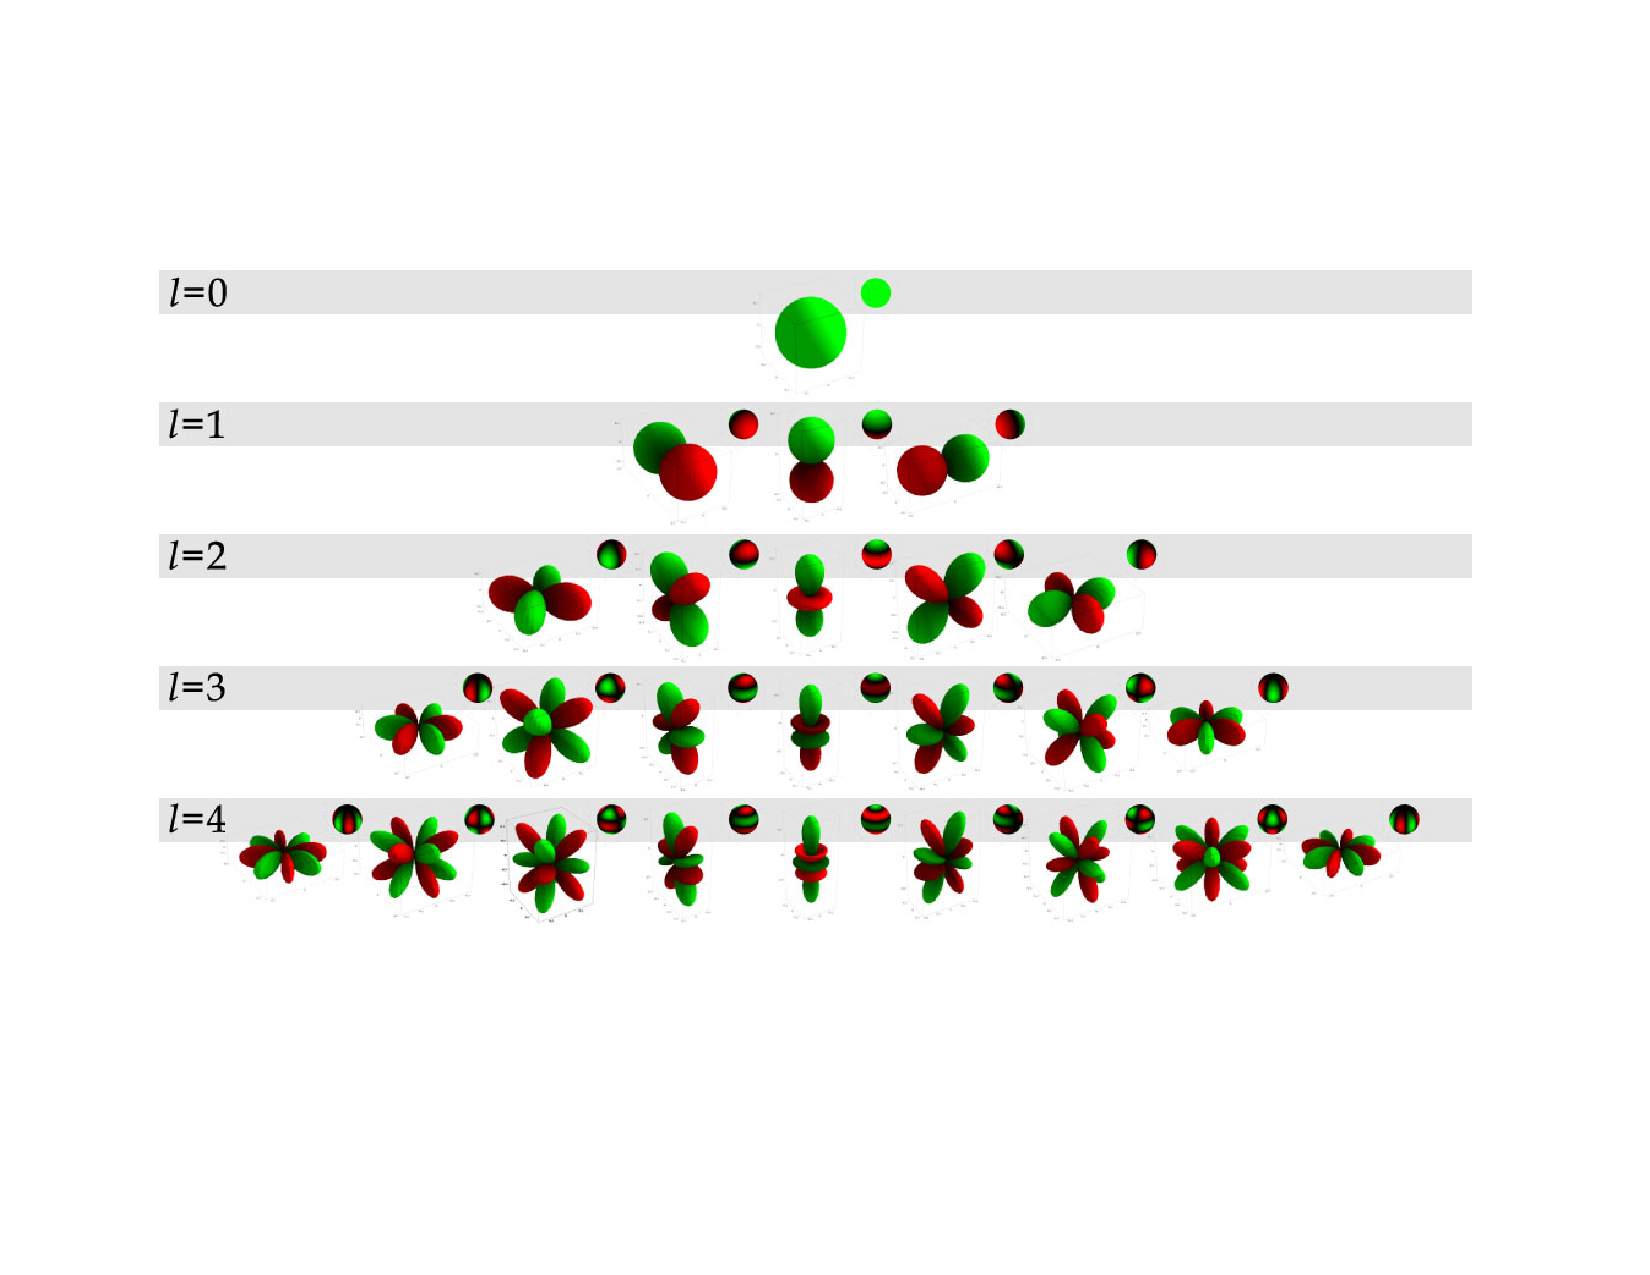
\includegraphics[width=1.0\textwidth]{Img/sh-shape.pdf}

    \caption[球形谐波基函数的形状]{ 
        球形谐波基函数的形状
        \label{fig:sh-shape}
        \cite{green2003spherical}
    }
\end{figure}

场景的光照分布可以映射到一个球面上,即$L(s)$, $s$ 表示从球心到球面上的一个方向。
通过SH基函数可以将球面上的光照分布映射为SH系数:
\begin{equation}
    SH^m_l = \int\limits_{S}L(s)y^m_l(s)ds
\end{equation}

根据$l$和$m$的关系,可以看出,$l$阶SH需要$2l$个系数。将光照映射到$n$阶时,共需要$n^2$个SH系数。
因此对于$n$阶的SH系数,可以将$SH$展开为一维向量$SH_i, 0 \leq i < n^2$

球面上的$n$阶SH近似光照$\tilde{L}(s)$可以通过SH系数计算:
\begin{equation}
    \tilde{L}(s)=\sum_{l=0}^{n-1}\sum_{m=-l}^{l}SH^m_ly^m_l(s)=\sum_{i=0}^{n^2}SH_iy_i(s)
\end{equation}
HDR全景图像映射为SH系数时,需要先将HDR全景图像投影到球面上,随后再将球面上的光照分布映射为一组SH系数。考虑到深度神经网络强大的学习能力,本文使用了4阶SH来近似场景光照,此外由于光照信息包含了三个通道,因此共需要48个SH系数($4^2\times3$)。
\section{光照估计网络结构}
在本文的光照估计方法中,输入为两幅由前后置相机拍摄的相对图片,目标输出为48个SH系数。因此需要搭建一个从两幅图片预测出48个参数的深度卷积神经网络(CNN)。
该网络需要从图片中提取特征图,并使用全连接层回归出用以表示光照的SH系数。
本文仔细地设计了光照估计的卷积神经网络结构,如图\ref{fig:overview}所示。

\begin{figure}
    \includegraphics[width=1.0\textwidth]{Img/fig-overview.pdf}
    \caption[光照估计网络结果一览]{
        \label{fig:overview}
        光照估计网络结果一览。
        在训练阶段(蓝色区域+黄色区域),使用HDR全景图分别提取普通图片和SH系数分别作为网络输入和目标输出信息,并使用Render Loss\ref{sec:loss-function}作为监督信息。
        在测试阶段(蓝色区域),成对的图片输入到网络中直接预测光照对应的SH系数。
        网络结构由两部分组成,一部分是共享权重的特征提取层,另一部分是由卷积层和全连接层构成的光照估计网络。
   }
\end{figure}

该网络结构主要包含两个部分:第一部分提取两幅输入图像的特征,第二部分融合这些特征并预测SH系数。 

本文构建的HDR数据集虽然有近千张,但是对于训练神经网络来说还是略显不足,因此需要考虑使用预训练的网络和参数提取图像特征。在调研时发现,场景的光照分布与场景的类型密切相关(例如, 室外,室内,白天,夜晚等),因此在特征提取部分采用了Zhou预训练的场景分类网络\cite{zhou2017places},这个网络在大规模数据集上进行了训练,有可能提取出较好的图像特征。 在预测回归阶段,提取的两组图像特征在通道维度被拼接在一起,随后经过卷积层和FC层,最终回归出SH系数, 表\ref{table:cnn}展示了详细的网络结构,除了最后一层外,其它层之后都有batch normalization和leaky RELU激活函数层。
\begin{table}[htbp]
    \centering
    \caption[光照估计网络结构]{
        \label{table:cnn}
        光照估计网络结构。该网络分为两个部分,首先特征提取层从输入图片中提取特征图,之后特征图会在通道层拼接(concatenate)在一起。紧接通过5个卷积层和6个全连接层输出48个球形谐波系数,除最后一层外,每层后都会有batch normalization 和 Leaky RELU激活函数。
    }
    \begin{tabular}{c|c|c} 
    \hline
    ~           &    View 1 & View 2    \\
    \hline
    Input       &   $224\times224\times3$  &    $224\times224\times3$ \\
    \hline
    Feature Extraction & \multirow{2}{*}{$5\times5\times256$} & \multirow{2}{*}{$5\times5\times256$}\\
    Network&~&~\\
    \hline
    Concat & \multicolumn{2}{c}{$5\times 5\times 512$}     \\
    \hline
    Convs $3\times3$     & \multicolumn{2}{c}{$5\times5\times64$}\\
    \hline
    Dense Layers          & \multicolumn{2}{c}{$2048$->$1024$->$512$->$256$->$128$}\\
    \hline
    Output      & \multicolumn{2}{c}{$16\times3$}\\
    \hline
    \end{tabular}
\end{table}

\section{损失函数}\label{sec:loss-function}
在训练神经网络时,损失函数的意义重大。合理的损失函数能够加快网络的收敛,提高网络的表现。本文通过分析SH和渲染结果之间的差异,提出了一个新的用于优化光照估计神经网络的损失函数。
\subsection{球谐参数损失函数} 为了预测的SH系数与真实SH系数之间的差异,一个比较直观的做法是使用MSE作为损失函数。不过在SH系数中,不同阶的参数个数是不同的,每一个SH系数在近似光照时所占的权重并不相同。为了平衡这种不均衡的权重,需要先在每一阶的SH系数上计算MSE,然后再不同阶之间做均值。这种均衡化之后的SH距离可以作为训练网络的损失函数。SH Loss的定义如公式\ref{eq:sh-loss}
\begin{equation}
    \mathcal{L}_{SH} = \frac{1}{n}\sum_{l=0}^{n-1}(\frac{1}{2l+1}\sum_{m=-l}^{l}(SH^m_l - SH^m_l)^2))
    \label{eq:sh-loss}
\end{equation}
其中,$n$为近似光照所使用的SH的阶数,该公式为每个颜色通道上的SH Loss,在整个颜色空间中对每个通道的Loss做均值即可。

\subsection{渲染结果损失函数} 虽然MSE是评估两个向量之间距离的常用指标,但是对于光照估计问题来说,仅用MSE来作为损失函数优化SH系数是不够的。实际上,较低的SH误差并不能保证对应光照的渲染结果足够好。SH系数上的微小差异也可能会导致渲染结果上非常大的误差。图\ref{fig:sh-render-diff}展示了一个比较SH系数和渲染结果差异的实验,该实验首先选取一张HDR全景图,然后每隔5\doge地水平旋转该HDR全景图,每次旋转记为一帧;对于每一帧,计算当前帧HDR全景图对应的SH系数,同时使用HDR渲染一个三维物体;通过分别计算当前帧的SH系数和渲染结果与前一帧的差异,绘制了SH系数差异和渲染结果差异之间的关系图。图中可以看出,经过5\doge的旋转,虽然SH之间的差异非常小,但是渲染结果的变化却十分巨大。因此需要在训练时对渲染结果进行监督。
\begin{figure}
    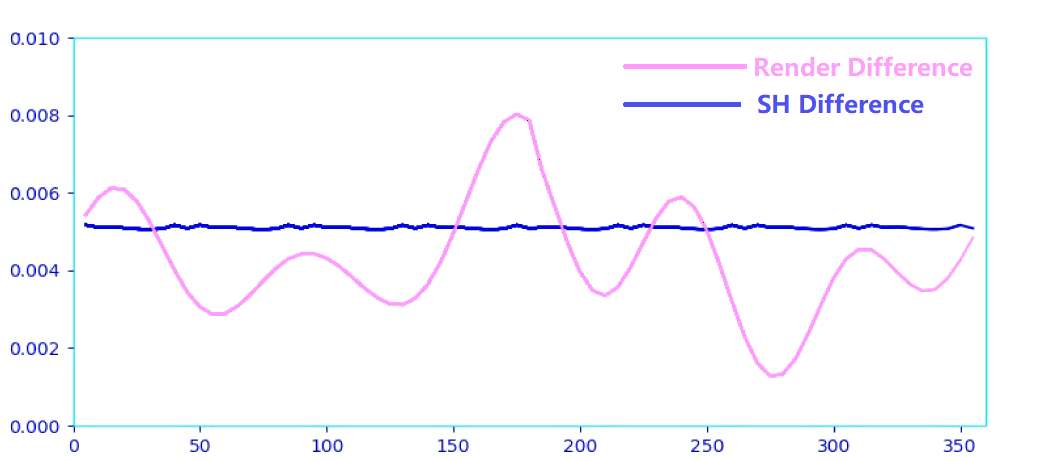
\includegraphics[width=1.0\textwidth]{Img/sh-render-diff.png}
    \caption[SH系数与渲染结果之间的不一致性]{
        \label{fig:sh-render-diff}
    每隔5\doge地旋转一幅HDR全景图,计算对应的SH系数,随后分别使用旋转后的HDR全景图和SH渲染一个物体,并计算他们之间的差异,它们之间的差异分布如图。
    }
\end{figure}


因此本文提出一种Render Loss,意图在训练光照估计神经网络时,增加渲染结果上的监督信息。具体的做法是先将一些3D物体渲染为一张SH Map(渲染方式参考\cite{green2003spherical})。使用SH Map与近似光照的SH系数可以计算出该光照下物体的渲染图像:
\begin{equation}
    R(SH, x, y, c) = \sum^{n^2}_{i=1}SHMap(x,y,i)*SH_{c,i}
\end{equation}

其中$n$为近似光照所使用的SH的阶数,$c$表示渲染图的某个通道, $(x, y)$为渲染结果和SH map的图片坐标。

上述公式表明,在预计算SH map之后,SH系数与渲染结果之间是线性的乘加关系,可以将其添加在神经网络中并计算梯度。因此可以定义Render Loss:
\begin{equation}
    \label{eq:render-loss}
    \mathcal{L}_{render} = \frac{1}{W\times H\times C} \sum_{x=1}^{W}\sum_{y=1}^{H}\sum_{c=1}^{C}(R(SH,x,y,c)-R(\hat{SH},x,y,c))^{2}
\end{equation}

其中$R(SH,x,y,c)$ SH的渲染结果在坐标$(x,y)$,通道$c$的颜色值。$W, H$ 分别是渲染图像的宽高,$C=3$表示RGB三个通道数。
最终的损失函数定义为SH Loss和Render Loss的加权和:
\begin{equation}
    \label{eq:loss-function}
    \mathcal{L} =w_{1}*\mathcal{L}_{SH}+w_{2}*\mathcal{L}_{render}
\end{equation}

 其中 $w_1$ 和 $w_2$ 是用来平衡 $\mathcal{L}_{sh}$和$\mathcal{L}_{render}$权重的超参数。
\section{实验结果与评估}\label{sec:experiment}
为了验证本文的深度光照估计方法的有效性,本文设计了光照估计实验,对比了提出的光照估计方法与当前最先进的(SOTA)方法,实验结果表明本文方法在室内室外场景下均优于其他方法。同时,该方法在真实场景下进行了测试,也获得了比较理想的结果。
\subsection{实现细节}
\begin{itemize}
    \item \textbf{数据准备} 通过拍摄和收集,本文构建了包含近千张HDR全景图的数据集。在训练光照估计网络时,需要使用这些HDR全景图生成大批量的训练和测试数据。首先HDR全景图按照90\%, 5\%, 5\%的比例划分为训练集,测试集和验证集,训练集用来训练光照估计网络,测试上的结果用来指导网络的超参数调整。验证集用以评估光照估计网络的表现。
    
    接下来生成输入图片。首先将划分后的每张HDR全景图映射到单位球体的表面,并将视点置于球心,然后选取一个视线方向$(\theta, \phi)$。根据球面坐标系的定义可知其相对方向为$(\pi-\theta, -\phi)$,这两个方向上的视图可以视为前后摄像头拍摄的两幅照片。由于大部分智能设备的前后置相机并不会很好的对齐,选取相对方向时,在垂直和水平方向分别添加了一个标准差为5\doge的高斯扰动。同时,为了通过数据增强提高光照估计神经网络的泛化能力,在提取图片时会使用随机的曝光值$e$,即HDR全景图乘以$2^e$,其中$e$服从[-1.5, 1.5]之间的均匀分布。

    在选取好方向$(\theta, \phi)$之后,该方向上的SH系数也可以被提取出来,该实验使用4阶的SH来近似场景光照,因此这里SH的系数共有48个($4^2\time3$通道)。
    
    对于每张HDR全景图,会均匀地随机128个方向来提取图片和SH系数,在过滤掉过度曝光和欠曝光的图片后,用于训练光照估计网络的图片/SH系数数据对大概为12万组。此外,数据的划分是在HDR全景数据集上进行的,所以同一幅HDR图像不会同时出现在训练集、测试集或验证集中,规避了训练集和测试集中包含相同图片的可能。
    \item \textbf{训练细节}训练光照估计网络的硬件平台、操作系统、优化器、学习率等参数列于表\ref{table:traning-details}中。另外在训练时,用以平衡$\mathcal{L}_{sh}$和$\mathcal{L}_{render}$权重的$w_1$ 和 $w_2$被设为0.8和0.2,这是通过探究实验(小节\ref{sec:ablation-study})获取的最佳配置。
    \begin{table}[htbp]
        \centering
        \caption{
            \label{table:traning-details}
            光照估计网络的训练细节。
        }
        \begin{tabular}{r|l}
            \hline
            项目 & 配置\\
            \hline
            硬件平台 & 处理器Intel6800k, 内存16G,显卡NVIDIA GTX 1080\\
            操作系统 & Ubuntu 18.04 64位\\
            优化器    & RMS Prop 优化器\\
            批大小    & 16,又称batch size\\
            初始学习率 & 0.0005 \\
            学习率衰减 & 每训练2万步,学习率乘以0.9\\
            训练时间 & 100个epoch,约1200万对数据,750万步\\
            \hline            
        \end{tabular}
    \end{table}
    \item \textbf{评估方式} 评估光照估计的常用方式是计算真实渲染结果(通常是图像)与估计光照渲染结果之间的差异。衡量图片之间距离的常用度量指标有均方差(mean squared error,MSE)、均方根(root mean squared error, RMSE)、平均绝对误差差(mean absolute  error,MAE)、结构相似性(structural similarity, SSIM)、结构差异性(structural dissimilarity, DSSIM)、峰值信噪比(peak signal to noise ratio,PSNR)等等。与现有的光照估计方法类似,本实验中选用的指标为RMSE和DSSIM。对于验证集中的每一对数据,真实的渲染结果使用原始的HDR全景图进行渲染,将其作为ground truth与使用预测SH渲染的结果对比,计算它们之间的RMSE和DSSIM,最后使用验证集上所有的RMSE和DSSIM均值作为评价光照估计方法的最终指标。
\end{itemize}
\subsection{与最先进方法的对比}
\begin{table}[t]
    \centering
    \begin{tabular}{c|c|c|c|c} 
    \toprule
    Image&Metric&Ours&[HGSH]&[GSY]\\
    \hline 
    \multirow{2}{*}{Indoor} &RMSE&\textbf{0.1437} & 0.1676 & 0.2182\\
                          ~&DSSIM&\textbf{0.0729} & 0.0759 & 0.1065\\
    \hline
    \multirow{2}{*}{Outdoor}&RMSE&\textbf{0.1185} & 0.1609 & 0.1984\\
                          ~&DSSIM&\textbf{0.0670} & 0.0780 & 0.0985\\
    \hline
    \multirow{2}{*}{Total} &RMSE&\textbf{0.1239} & 0.1622 & 0.2027\\
                         ~&DSSIM&\textbf{0.0686} & 0.0776 & 0.1003\\
    \bottomrule
    \end{tabular}
    \caption[本文方法与最先进方法的对比]{

        \label{table:cmp-previous}
        与最先进的方法进行定量比对,Hold-Geoffroy等人\cite{hold2017deep}和Gardner等人\cite{gardner2017learning}的工作分别适用于室外和室内图像。 本文的结果在数值上超过了这两个方法。
    }
\end{table}
本文与目前的两个最先进的(state-of-the-art, SOTA)光照估计工作进行了对比:Hold-Geoffroy等人\cite{hold2017deep}的室外光照估计工作,Gardner等人\cite{gardner2017learning}的室内光照估计工作。前者通过卷积神经网络,从室外图片预测出sun-sky模型\cite{hovsekhovsek2013adding}的几个物理参数,进而达到估计光照的目的;后者通过在大规模低动态范围全景图上预训练、在小规模室内高动态范围全景图上微调(fine-tune),构建了一个从室内图片预测场景光照的深度学习模型;这两个工作都提供了从图片到HDR全景图的在线应用,上传一张图片后就可以获取估计的光照分布。在验证集上,本文方法与这两个工作进行了对比,数值结果如表\ref{table:cmp-previous}所示。可以看出,无论是室外场景还是室内场景,本文方法在RMSE和DSSIM两个指标上均明显优于其它工作。图\ref{fig:cmp-previous}是本方法和两个SOTA方法的可视化对比,结果显示是用本文方法估计的光照渲染的3D物体更接近真实的渲染结果。
\begin{figure}
  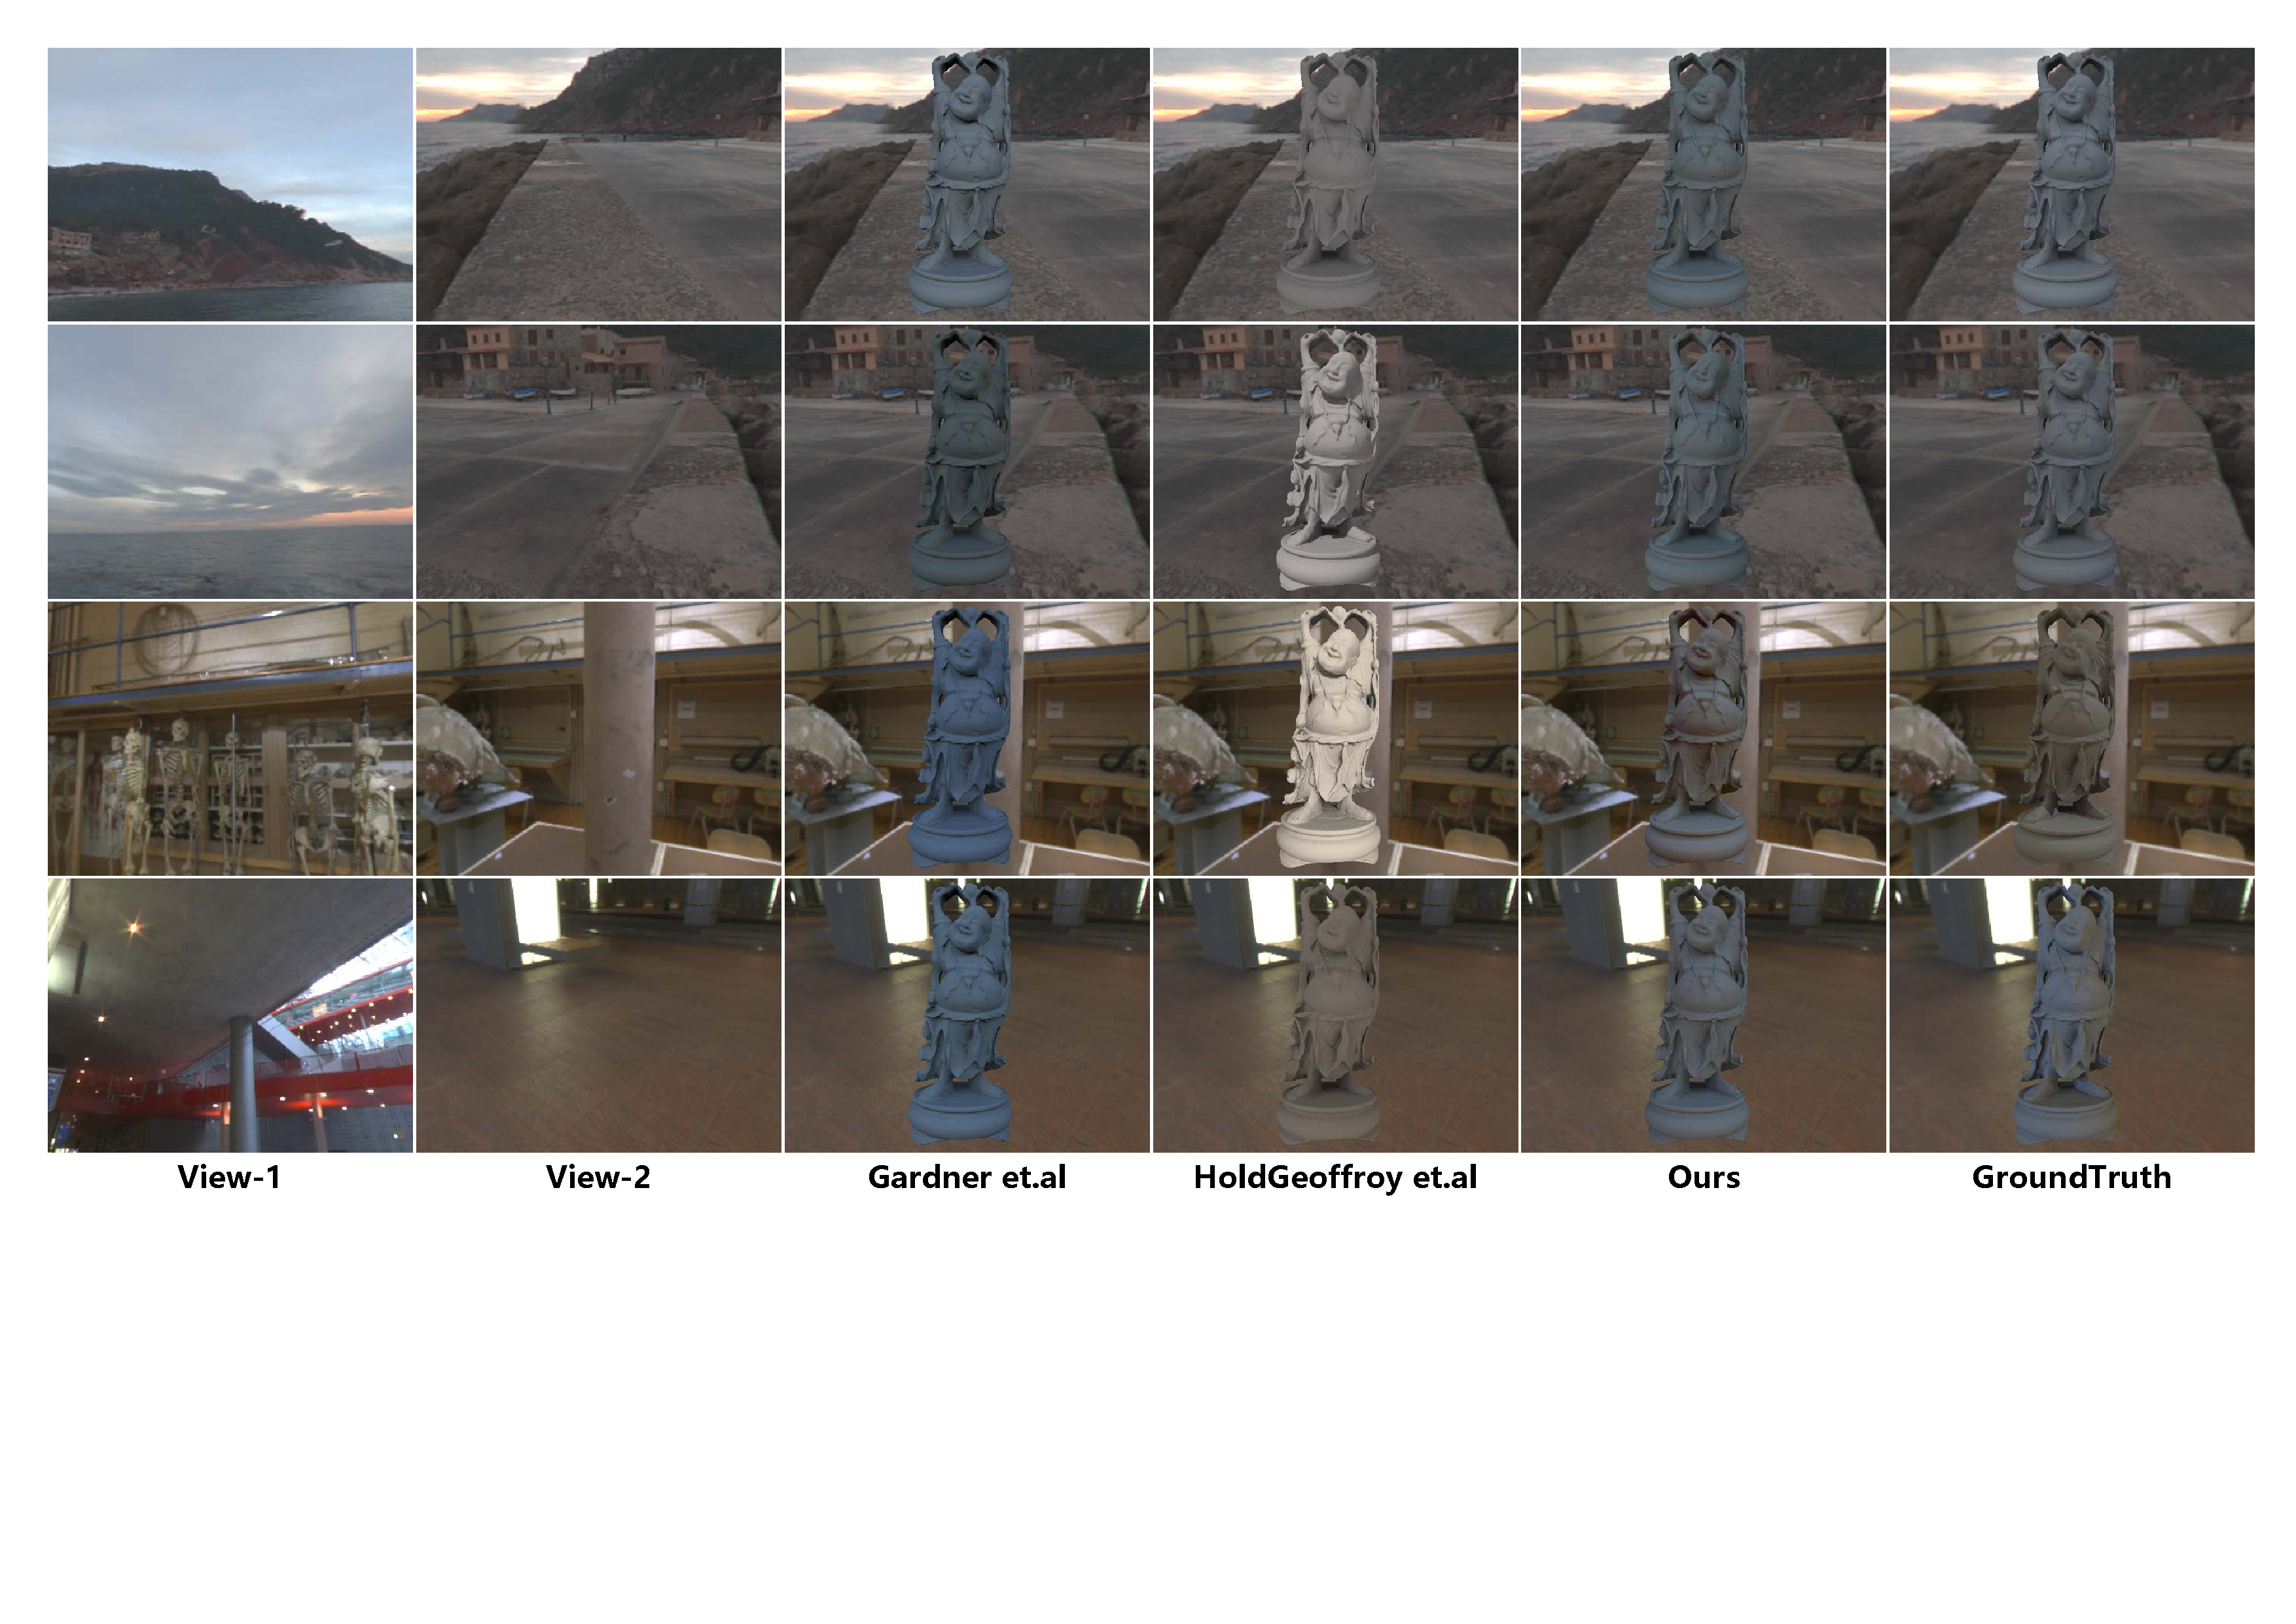
\includegraphics[width=1.0\textwidth]{Img/fig-cmp.pdf}
  \caption[与最先进方法的对比]{
    \label{fig:cmp-previous}
    本文工作与Gardner等人\cite{gardner2017learning}、Hold-Geoffroy等人\cite{hold2017deep}两个最先进方法的对比。可以看出,本文的方法在室内和室外场景中结果均优于这两个方法。
  }
\end{figure}

\subsection{在真实数据上的表现}
本文的光照估计方法使用视角相对的两张图片作为输入,这对于具有前后相机的现代设备来说有着实际的意义。因此本文测试了该光照估计方法在真实场景中的表现。用于测试的设备是一部普通的智能手机和一台全景相机。首先使用智能手机的前后置相机同时拍摄两张图片,然后使用全景相机在同样的位置获取HDR全景图。拍摄的两张图片输入到光照估计网络,随后使用预测的SH系数渲染一个3D物体插入到图像中,最后将此结果与使用HDR全景图渲染的结果进行对比。图\ref{fig:realphoto}展示了本文方法在真实场景中的表现,可以观察到本文方法在多种场景下均能取得较好的预测结果。

\section{深入研究光照估计网络}\label{sec:ablation-study}
本文方法中的网络结构包含了多个模块:特征提取模块,特征融合模块,光照估计模块等等,训练过程中也有多个可调的参数,例如损失函数中的权重系数$w_1$和$w_2$。这些模块和参数的选取与使用方式都在一定程度上影响了光照估计效果。本节通过几十组详细的实验,探究这些模块、参数对光照估计结果的影响,从可视结果与数值结果上就行定性和定量的分析。这些实验和分析对以后的深度学习、光照估计工作来说有着一定的指导意义。
\begin{figure*}
  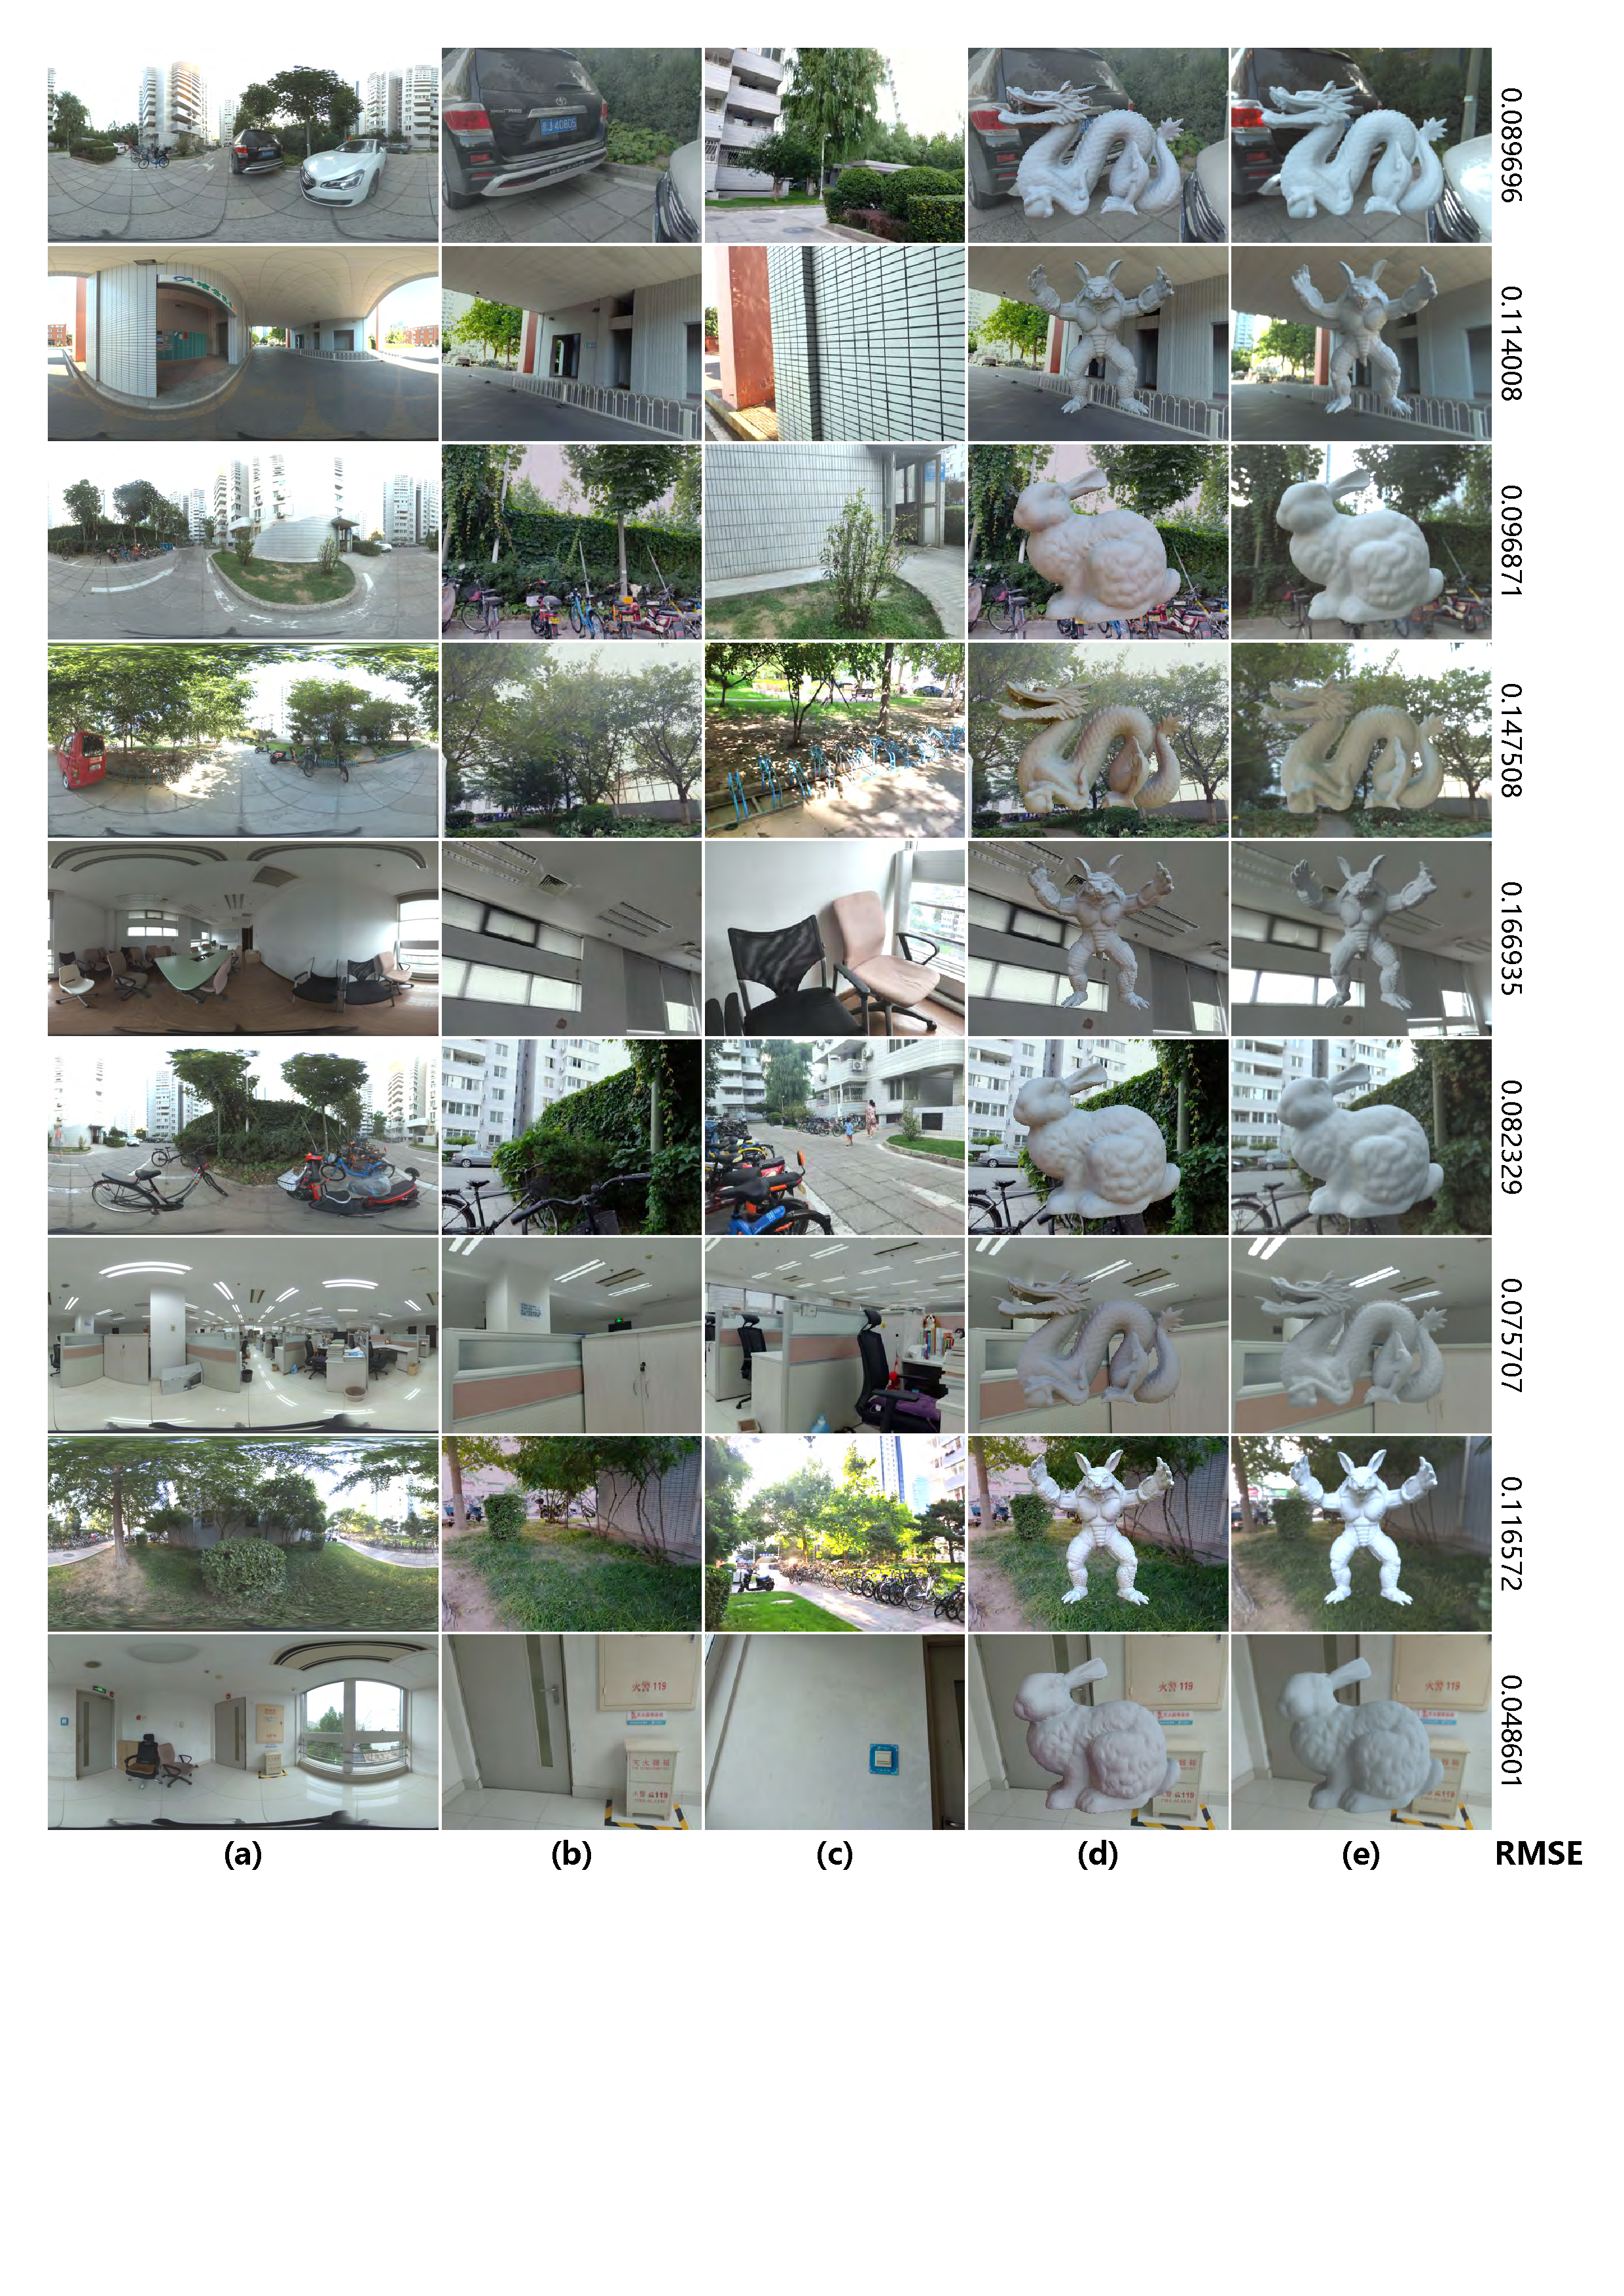
\includegraphics[width=1.0\textwidth]{Img/fig-realphoto.pdf}
  \caption[本文方法在真实场景中的结果]{
    \label{fig:realphoto}
      本文方法在真实图像上的估计结果。(a)场景的HDR全景图;(b)前置摄像头的图像;(c)后置摄像头的图像;(d)预测结果;(e)来自HDR全景图渲染的参考图像。
      由于真实场景中输入图片和HDR全景图并不是使用一个设备拍摄的,为了得到输入图片对应的真实渲染结果,需要手动对齐输入图像与HDR全景图,这导致了它们之间有一些小的偏移,不过这对于结果评估来说没有影响。
      结果显示本文方法在真实场景中也能取得很好的预测结果。
  }
\end{figure*}
\subsection{探究特征提取模块}
在光照估计网络中,特征提取模块使用的是Zhou等人\cite{zhou2017places}的场景分类网络结构。不过Zhou等人\cite{zhou2017places}在进行场景分类时,使用了多种类型的网络模型,例如AlexNet\cite{krizhevsky2012imagenet},GoogleNet\cite{szegedy2015going},VGG-16\cite{simonyan2014very}等。即使使用同样的数据和训练方式,这些网络在场景分类时也有着不同的表现。使用不同的网络作为光照估计网络中的特征提取模块,也会极大地影响光照估计的效果。因此需要通过实验对比使用不同的网络结构时结果的差异。

\begin{table}[ht]
    \centering
    \caption[不同特征提取网络的对比]{
    \label{table:backbone}
    使用不同特征提取网络的结果比较,评价指标采用RMSE和DSSIM。 对于每种网络结构,使用三种方式来评估网络性能:(a)从头开始训练整个网络(train from scratch); (b)从预训练模型中微调(fine-tune)。 (c)固定特征提取网络的预训练参数,仅训练照明估计网络(freeze)。 结果表明,在不同网络中处理特征提取网络的最佳方式是不同的。 这取决于采用的骨干模型以及训练数据的大小。 基于此表格,我们使用固定参数的AlexNet作为特征提取网络。
    }
    \begin{tabular}{c|c|c|c|c|c|c} 
     \hline
    \multirow{2}{*}{}  & \multicolumn{2}{c|}{GoogLeNet} & \multicolumn{2}{c|}{VGG-16} & \multicolumn{2}{c}{AlexNet} \\ \cline{2-7}
    ~&RMSE&DSSIM&RMSE&DSSIM&RMSE&DSSIM\\
    \hline
    (a) & 0.1304 & 0.0656 & 0.1269 & \textbf{0.0642} & 0.1638 & 0.0799 \\
    (b) & \textbf{0.1292} & \textbf{0.0656} & \textbf{0.1303} & 0.0661 & 0.1318 & 0.0717 \\
    (c) & 0.1329 & 0.0696 & 0.1336 & 0.0718 & \textbf{0.1239} & \textbf{0.0686} \\
    \hline 
    \end{tabular}
\end{table}
对于同一个特征提取网络,预训练的网络参数的使用方式也有多种:
\begin{itemize}
    \item \textbf{Freeze},固定住预训练好的网络参数。这种方式将直接使用预训练的参数进行特征提取,在训练整个网络时,这部分参数保持固定,不参与变量的更新。
    \item \textbf{Fine-tune}, 以预训练的网络参数作为初始参数。在训练的过程中与网络中的其它部分一起计算梯度,更新参数。
    \item \textbf{From scratch},不实用预训练的参数。这种方式只使用引入的网络结构,网络中变量使用随机的初始值,并参与网络中的变量更新。
\end{itemize}

对于不同的问题、模型、训练集,选取合理的预训练参数引入方式十分重要。
本节设计了九组实验,分别使用不同的网络结构和参数引入方式组合。表格\ref{table:backbone}展示了这些方式在验证集上的数值结果,选取的两个评价指标是渲染结果上的RMSE和DSSIM。可以看出,对于不同的网络结构,最佳的预训练网络参数的引用方式并不相同。对于GoogleNet和VGG-16这两种结构来说,最好的方式是fine-tune预训练参数。而对于Alexnet来说最好的使用方式是Freeze,即固定住预训练参数,其中的变量不参与参数更新。图\ref{fig:fix-backbone}展示了在不同的参数引入方式下,光照估计的结果对比,可以看出固定预训练网络参数的方式更接近真实的渲染结果。
\begin{figure}
  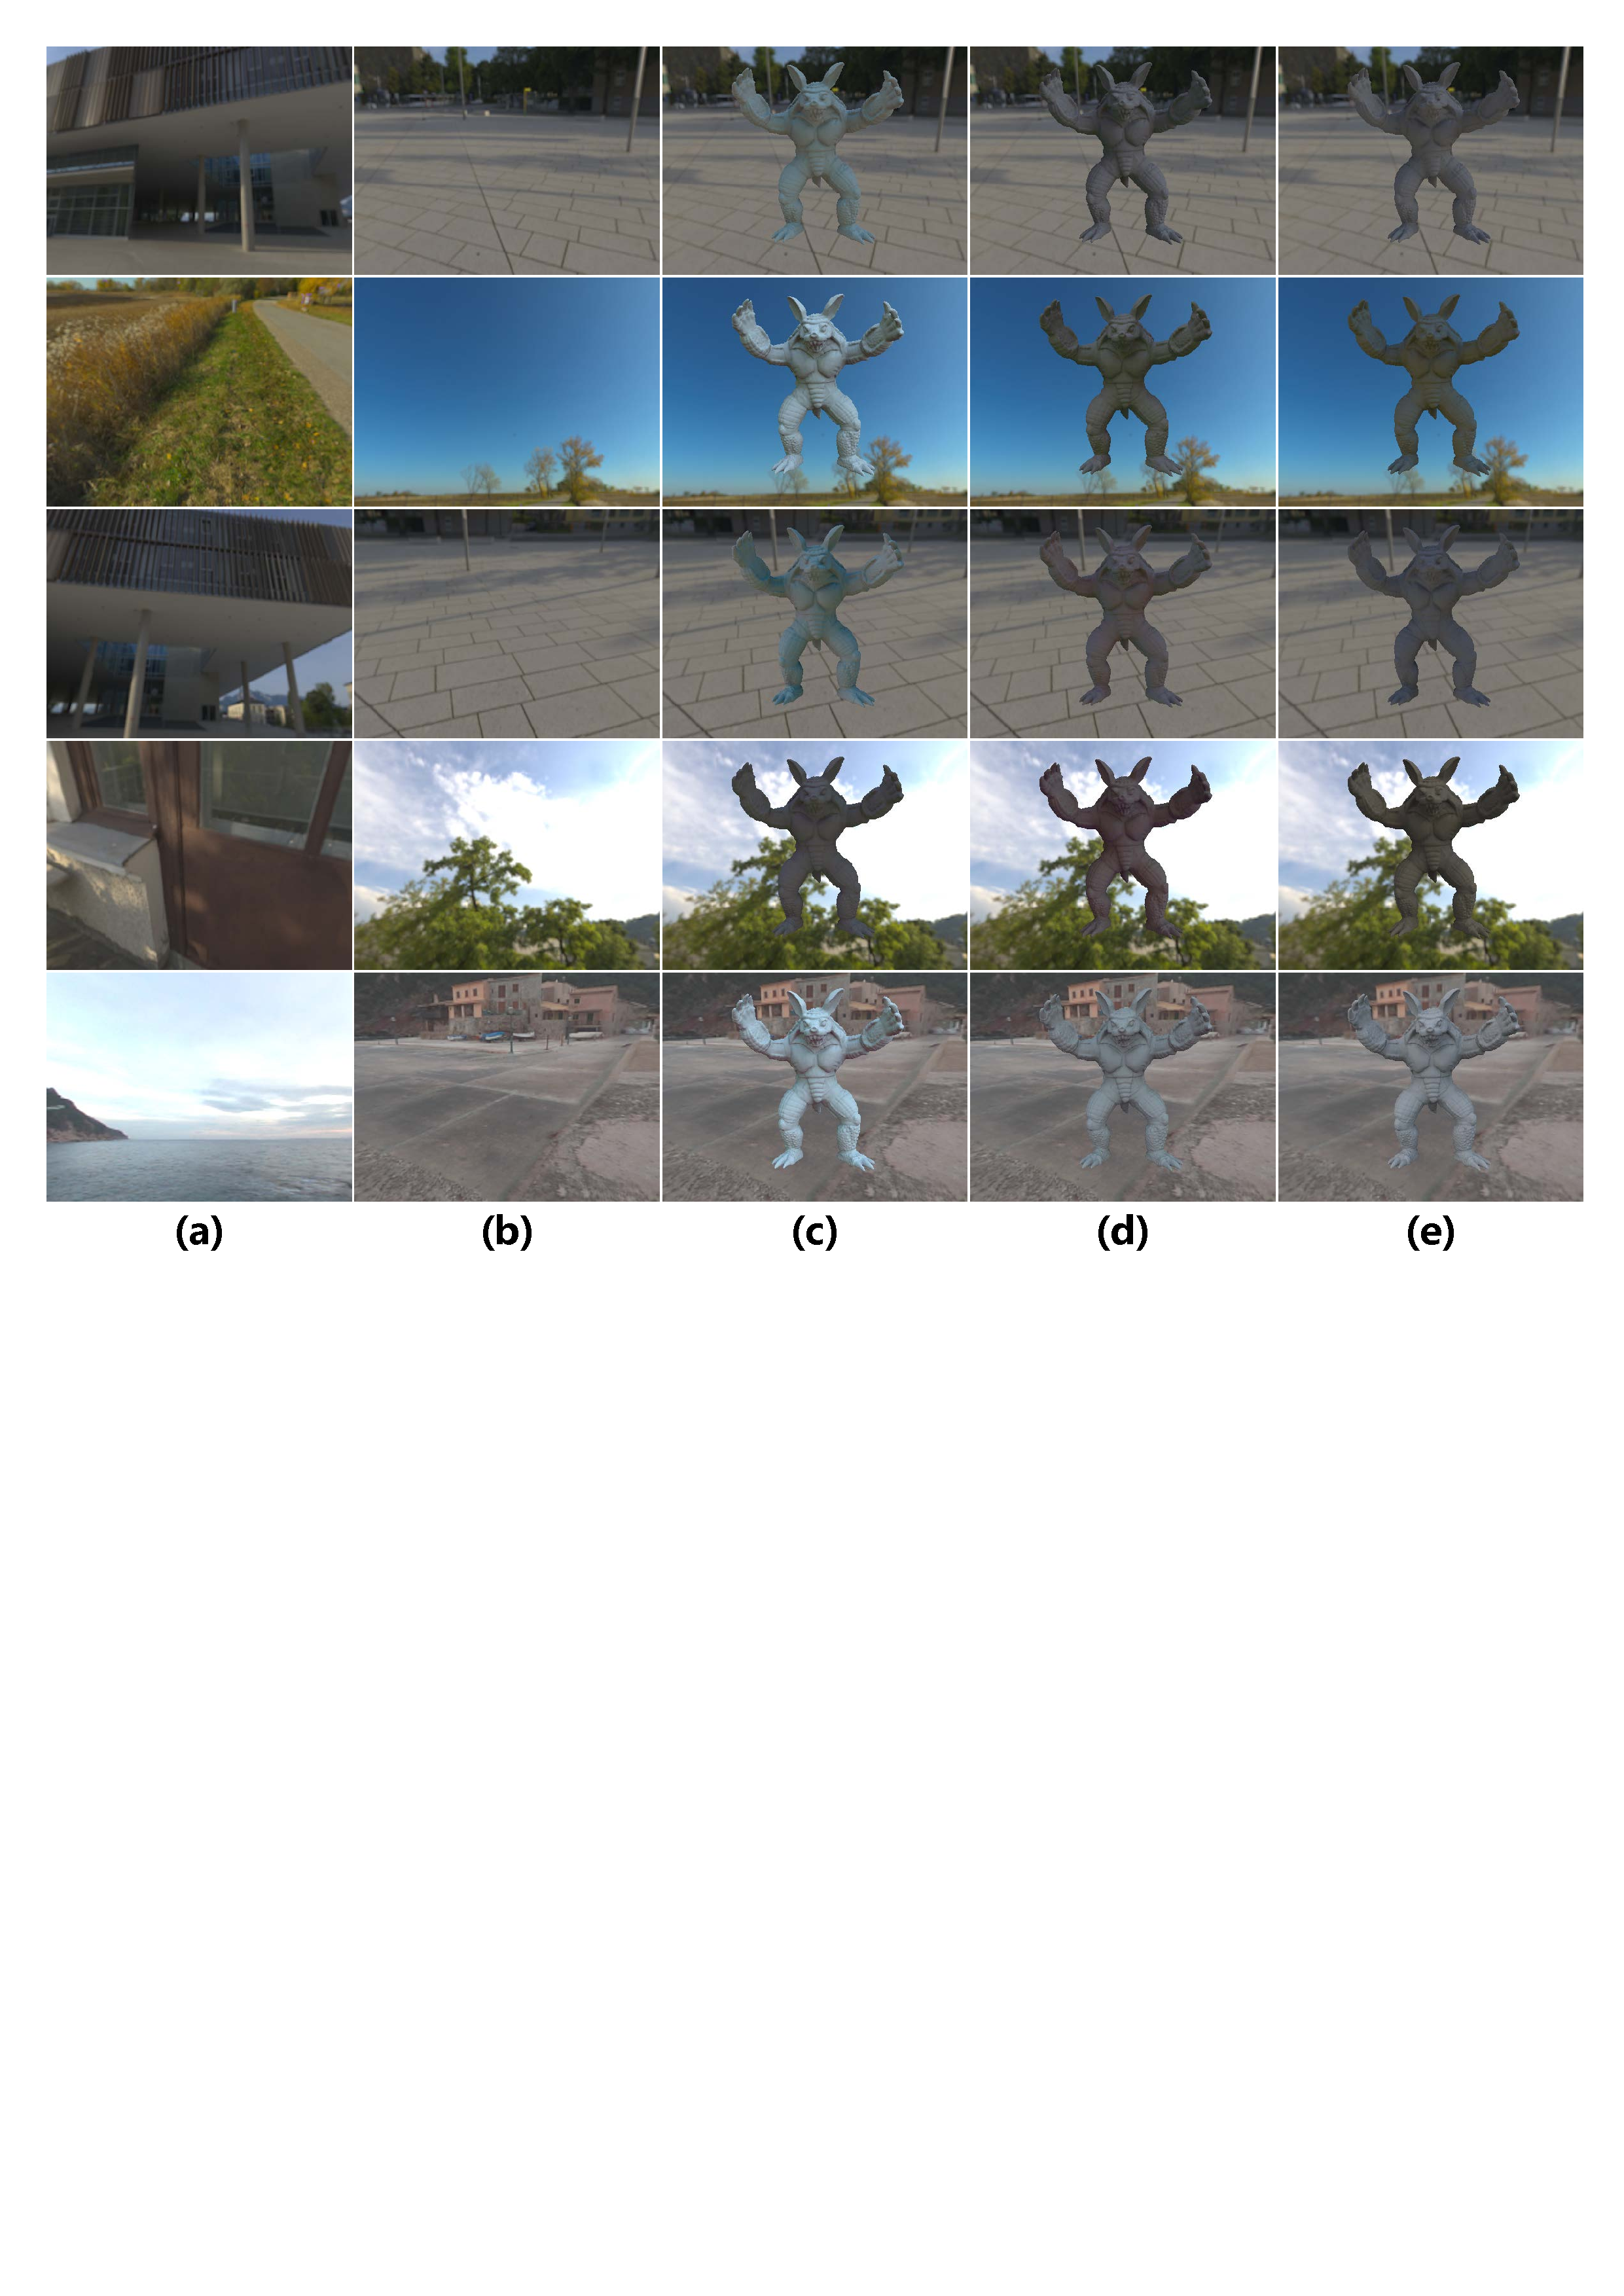
\includegraphics[width=1.0\columnwidth]{Img/fig-fixornot.pdf}
  \caption[不同的预训练参数引用方式对光照估计的影响]{
  \label{fig:fix-backbone}
  不同的预训练参数引用方式对光照估计的影响。(a)(b)输入图片;(c)Train from scratch的结果;(d)Freeze参数的结果;(e)真实渲染结果。
  }
\end{figure}

不过值得一提的是,目前的结果只是在当前数据集上的表现。由于数据集规模限制,如果不使用预训练参数,网络可能难以从有限的数据中学到足够好的特征选取方式,因此固定预训练参数的方式表现最好。在数据集扩充以后,最佳的参数引入方式极有可能发生变化,当然,这需要在以后研究中使用更大规模的数据进行更详细的验证。

在目前的数据集上,表现最好的网络结构与参数引用方式组合是使用固定参数的Alexnet,因此后续的探究中均使用这种结构和方式进行对比实验。
\subsection{探究特征融合方式}
\begin{table}[t]
    \centering
    \caption[特征融合方式对光照估计的影响]{
    \label{table:fusion-method}
    使用两种不同的方式融合特征提取层提取的两组特征图像,并对比它们之间的差异,结果显示在该方法中,特征拼接总是优于特征相减。
    }
    \begin{tabular}{c|cc|cc} 
     \hline
        ~&\multicolumn{2}{c|}{RMSE}&\multicolumn{2}{c}{DSSIM}\\
        Backbone & Concat & Sub. & Concat &Sub.\\
    \hline
    GoogLenet & \textbf{0.1329} & 0.1390 & \textbf{0.0696} & 0.0729 \\ \hline
    VGG-16    & \textbf{0.1336} & 0.1399 & \textbf{0.0718} & 0.0719 \\ \hline
    AlexNet   & \textbf{0.1239} & 0.1262 & \textbf{0.0686} & 0.0690 \\ \hline
    \end{tabular}
\end{table}

% \begin{table}[t]
%     \centering
%     \begin{tabular}{cc|cc|cc} 
%      \hline
%         ~&~&\multicolumn{2}{c|}{MSE}&\multicolumn{2}{c}{DSSIM}\\
%         Backbone & Method& Concat & Sub. & Concat &Sub.\\
%     \hline
%     \multirow{2}{*}{VGG-16}&(a) & \textbf{0.0088} &  {0.0096} & \textbf{0.0411}  & 0.0412\\
%     ~&(b)& 0.0104 & 0.0104 &0.0505  &  0.0511 \\
%     \hline
%     \multirow{2}{*}{AlexNet}&(a)& \textbf{0.0096}  & 0.0105 &  \textbf{0.0588} & 0.0592  \\
%     ~&(b)& 0.0112 & 0.0106 &0.0662 &  0.0737 \\
%     \hline
%     \multirow{2}{*}{ResNet-152}&(a)& \textbf{0.0090} & 0.0115 & 0.0502 & 0.0507   \\
%     ~&(b)& 0.0114  & 0.0103&  0.0517 & \textbf{0.0499} \\
%     \hline
%     \end{tabular}
%     \caption{
%     \label{table:fusion-method}
%     Comparison using different fusion layer for the convolutional feature maps of front and rear images. We use MSE and DSSIM for evaluation. (a)(b) mean two ways to use these backbones. (a) Freeze the feature extraction network and only train the illumination estimation network; (b) Train the entire network.
%     We find that the concatenation fusion with training strategy (a) is consistently better. 
%     }
% \end{table}
本文的光照估计网络的输入是两张图片,使用预训练的网络从这两幅图片中提取出两组特征图像后,需要将其进行合并才能输入到后续的网络中,因此需要选择合理的特征融合方式。常见的特征图融合方式都是在通道层进行的,例如通道层拼接、通道层相加、通道层相减、通道层相乘等等。深度学习任务中使用做多的特征融合方式是通道层拼接(concatenate)。

在该问题中,特征图在通道层相加是不合理的。由于两幅图片使用的是完全相同的特征提取网络,所以当融合方式是相加时,交换两幅图片产生的结果不会有任何变化,但实际上这两个方向的光照是截然不同的,这显然不合常理。而拼接和相减却没有这个问题,因此本节实验对比了这两种方式对光照估计结果的影响,实验结果如表\ref{table:fusion-method}所示,可以看出通道层拼接在各种网络结构和评价指标上均优于通道层相减。


\subsection{探究损失函数}
\begin{table}[ht]
    \centering
    \resizebox{\textwidth}{!}{
    \begin{tabular}{c|c|c|c|c|c|c|c|c|c|c} 
     \hline
    \multirow{1}{*}{($w_{1},w_{2}$)} & \multicolumn{2}{c|}{($0.0, 1.0$)}& \multicolumn{2}{c|}{($0.2, 0.8$)}& \multicolumn{2}{c|}{($0.5, 0.5$)}& \multicolumn{2}{c|}{($0.8, 0.2$)}& \multicolumn{2}{c}{($1.0, 0.0$)} \\ \cline{1-11}
    ~&RMSE&DSSIM&RMSE&DSSIM&RMSE&DSSIM&RMSE&DSSIM&RMSE&DSSIM\\ \hline
    GoogLeNet  & 0.1422 & 0.0742 & 0.1334 & 0.0712 & 0.1445 & 0.0785 & \textbf{0.1329} & \textbf{0.0696} & 0.1376 & 0.0732\\
    VGG-16     & 0.1447 & 0.0749 & 0.1561 & 0.0768 & 0.1587 & 0.0765 & \textbf{0.1336} & 0.0718 & 0.1656 & \textbf{0.0674}\\
    AlexNet    & 0.1247 & 0.0678 & 0.1268 & \textbf{0.0675} & 0.1479 & 0.0770 & \textbf{0.1239} & 0.0686 & 0.1267 & 0.0682\\
    \hline 
    \end{tabular}}
    \caption[损失函数对光照估计的影响]{
        \label{table:test-weight}
        使用具有不同权重配比的损失函数训练光照估计网络,并在测试集上分析它们之间的优劣。 其中$w_1$和$w_2$对应于公式\ref {eq:loss-function}中定义的权重系数。 我们可以观察到使用混合损失函数可以提高光照估计的性能。
    } 
\end{table}
为了探究提出的render loss对光照估计结果的影响,并找到最优的损失函数权重系数$w_1$,$w_2$(公式\ref{eq:loss-function}),本节设计和实现了十几组实验,详细地对比了使用不同的$w_1$,$w_2$的损失函数对光照估计结果的影响。表\ref{table:test-weight}列出了详细的实验结果,结果表明使用$w_1=0.8$,$w_2=0.2$的损失函数能够达到最好的结果。图\ref{fig:test-weight}的可视结果也表明,相较于只使用一类损失函数,综合使用两个损失函数可以得出更加接近真实值的效果。

\begin{figure}
  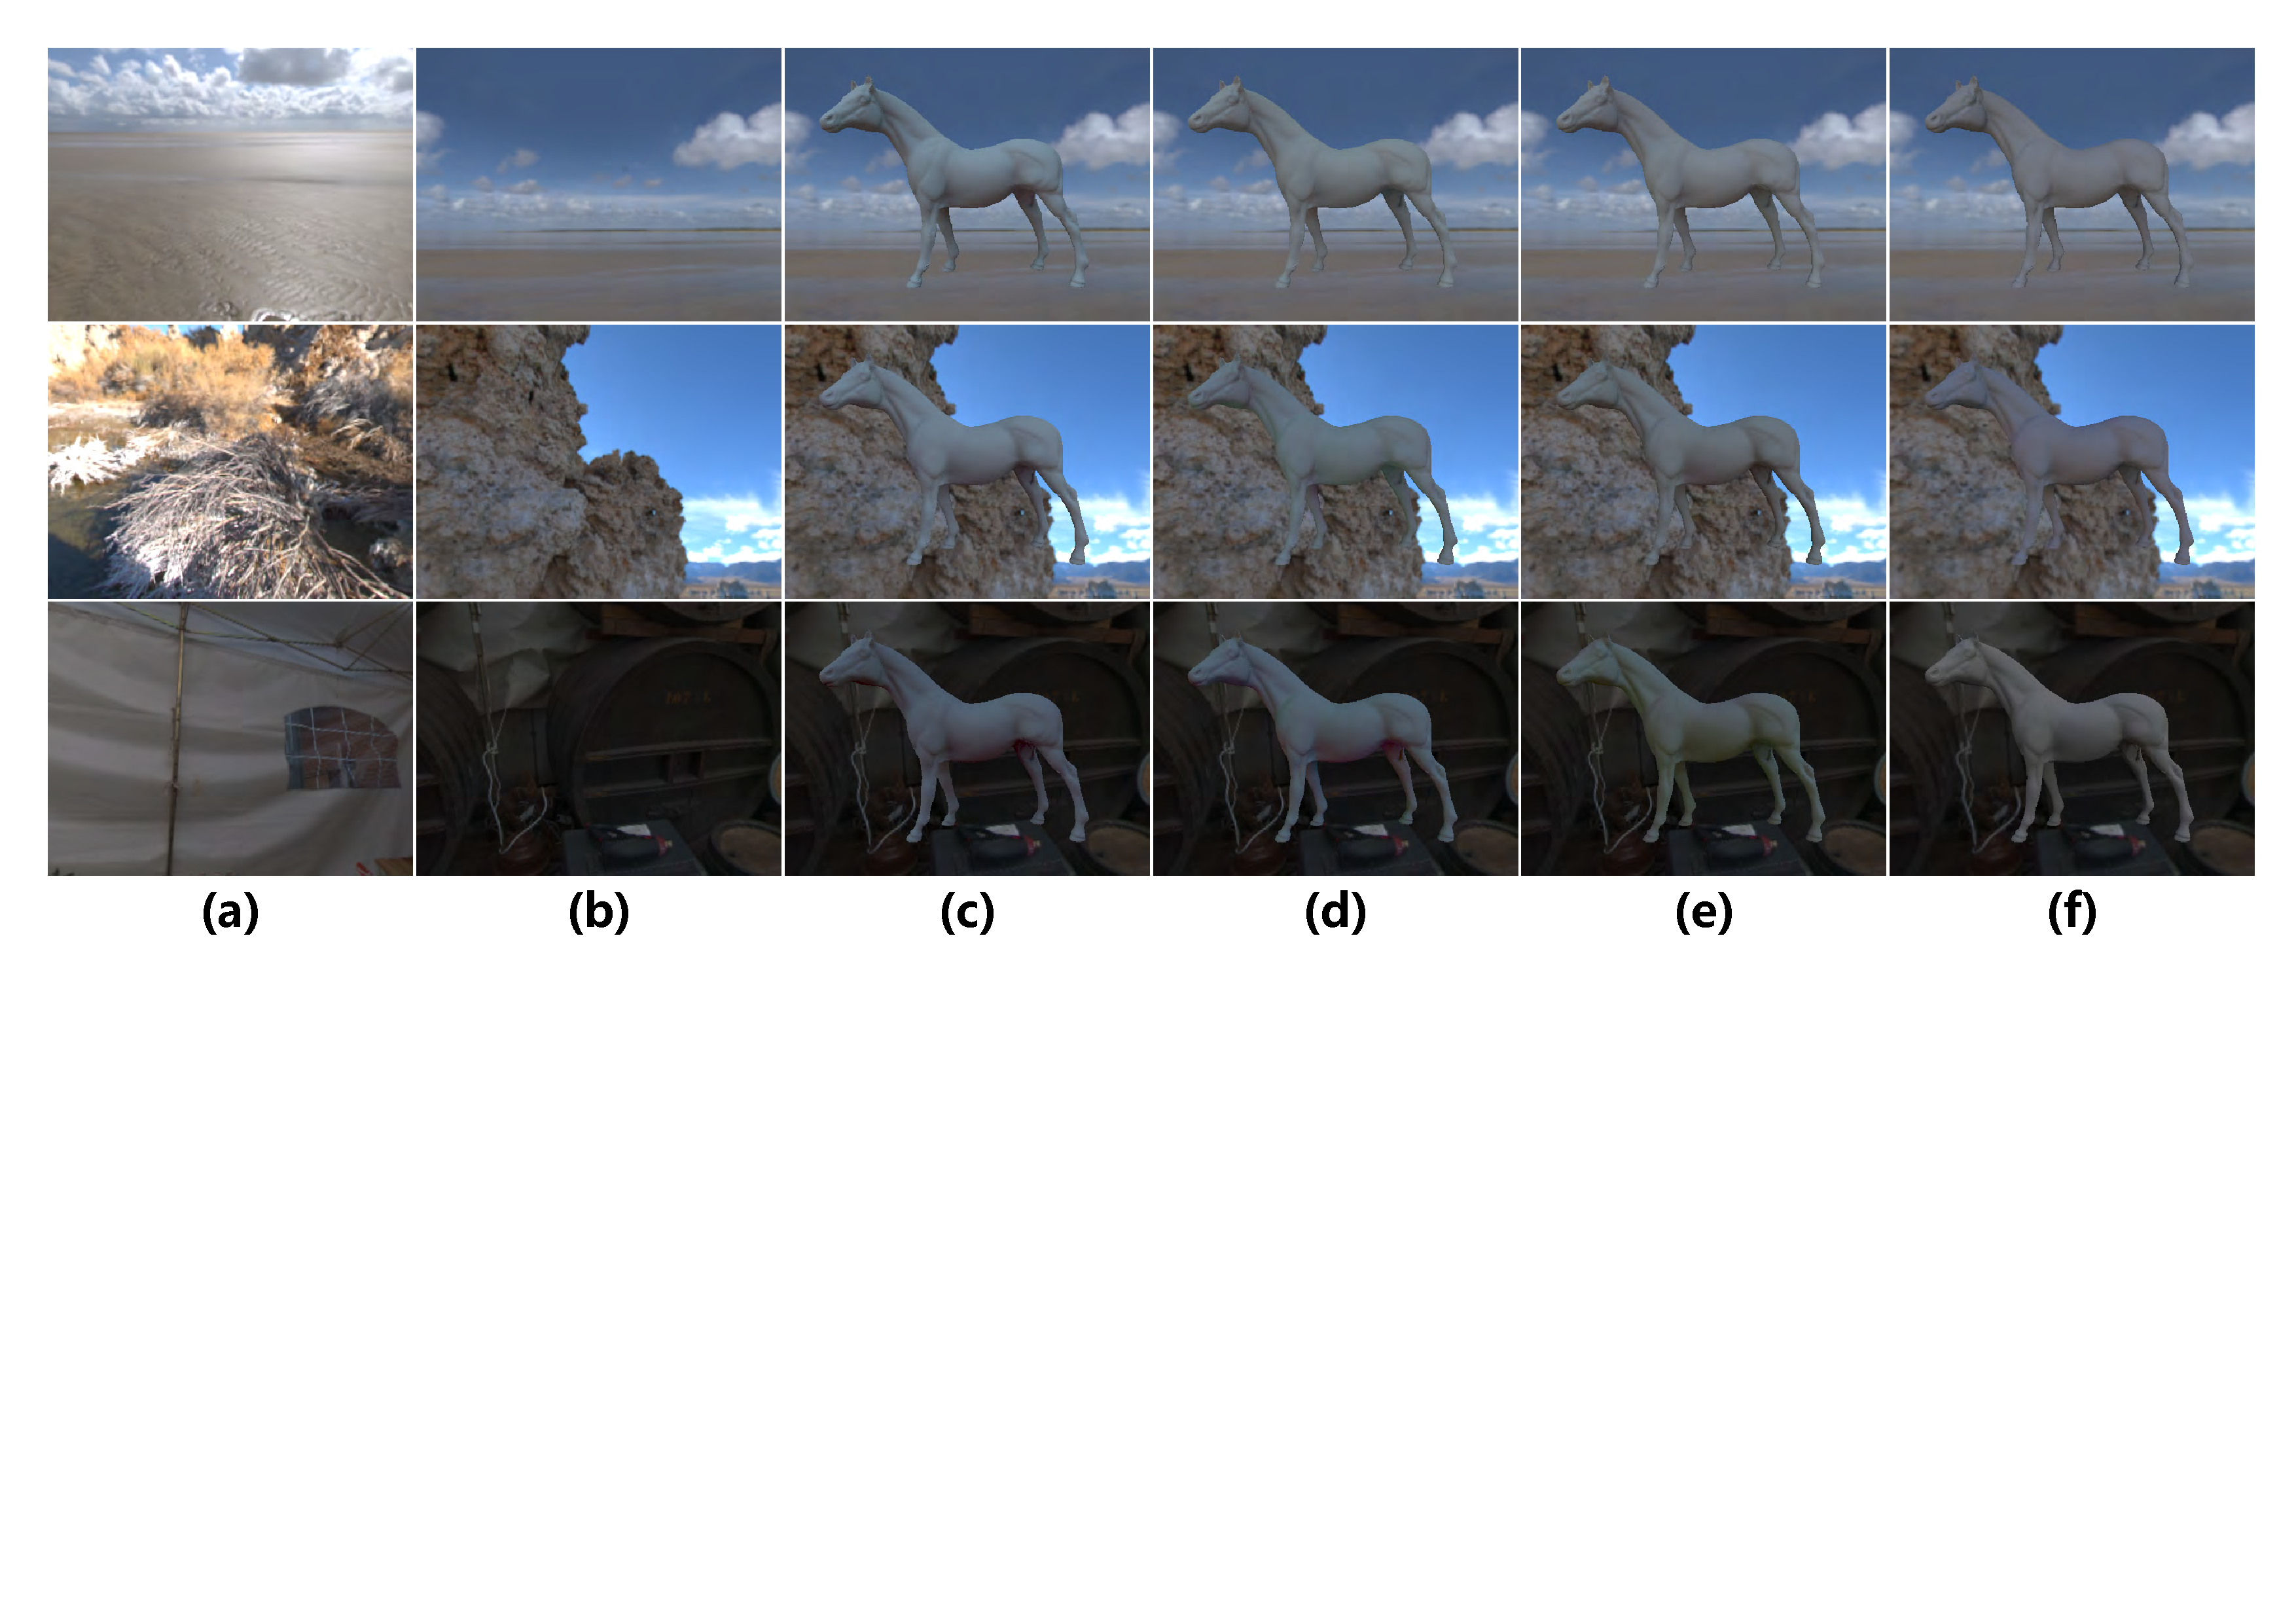
\includegraphics[width=1.0\textwidth]{Img/fig-test-weight.pdf}
  \caption[损失函数对光照估计的影响]{
    \label{fig:test-weight}
    损失函数对光照估计的影响。 (a)(b) 输入图像(c) 只使用SH Loss(公式\ref{eq:sh-loss});(d)只使用RenderLoss (公式\ref{eq:render-loss}); (e) 使用加权loss(公式\ref{eq:loss-function}); (f) 真实结果}
\end{figure}

需要注意的是,在训练时计算render loss所用的三维物体,与在测试时渲染的三维物体是不相同的。因此render loss能够提升效果的原因并不是来源于3D物体的先验知识,而是render loss本身对于渲染过程和场景光照的关注。这也是只使用render loss的效果比较差的原因之一。
\subsection{探究光照估计性能}
本文所提出的关照估计算法非常适合现代智能手机应用,因此模型的性能也是需要考量的一个因素。本文测试了光照估计的性能表现,在普通的消费级桌面显卡NVIDIA GTX 1080上,从一对图片估计出SH系数耗时0.0391秒,在CPU(INTEL i76800k)上则需要0.3039s。虽然该耗时无法在大量的低端设备达到实时,但是通过优化和裁剪仍然可以达到不错的交互速度。此外,目前的网络结构使用的是AlexNet,虽然该模型在当前数据集上最好的选择,但随着数据集规模的不断增加,一些轻量级的网络可能会更加合适。同时随着现代智能设备处理器性能的不断提高,该方法有望在移动设备中达到实时交互的效果。
\section{讨论}
本章提出了一个从图片恢复场景光照的深度学习模型。该模型使用现代智能设备的前后相机拍摄的图片作为输入,预测出场景光照分布对应的球形谐波系数。该网络由特征提取模块,特征融合模块,光照估计模块组成,其中特征提取模块引用了Zhou\cite{zhou2017places}的网络结构和参数。结合创新提出的损失函数render loss,该网络模型不仅能够获得超过最先进方法的结果,其在真实场景的表现也很理想。不过该方法仍然有一些局限性。一方面是使用SH表示光照的局限性,使用SH表示的光照往往会忽略掉一些高频信息,这对于具有镜面反射表面的物体来说很不友好。另一方面是仅使用图片预测光照时,对输入信息的依赖比较严重,如果输入图片既没有拍摄到场景的光照也没有拍摄到能推理出光照的阴影,则光照估计的效果很可能会不太理想。图\ref{fig:failure-case}展示了一种因为这两种局限性导致的失败情况。
\begin{figure}
  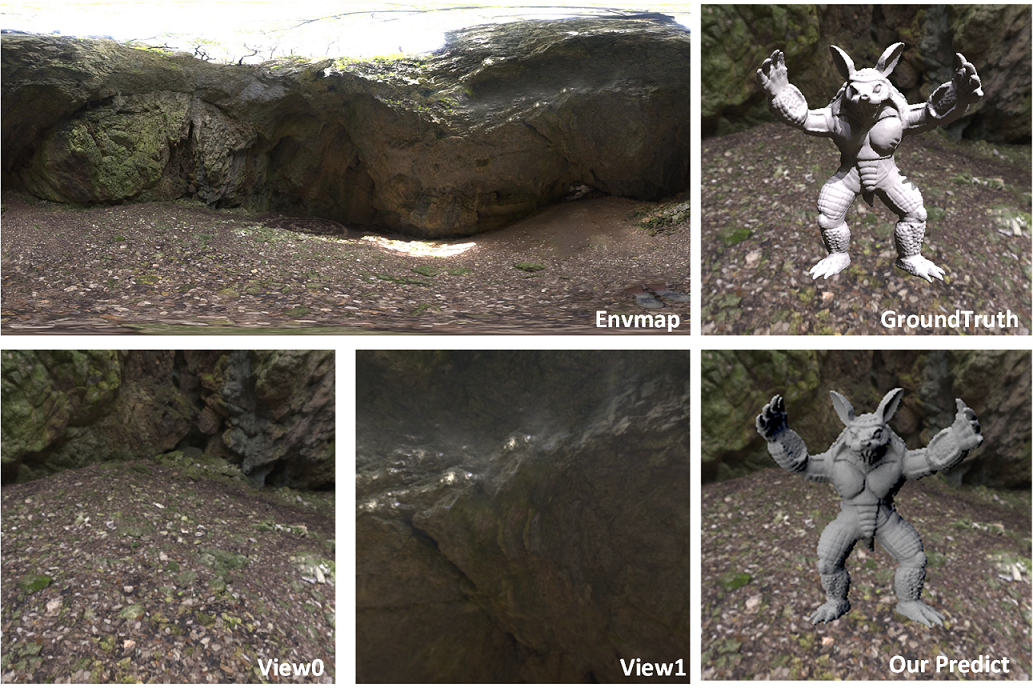
\includegraphics[width=\columnwidth]{Img/fig-failure.png}
  \caption[光照预测失败的例子]{
    \label{fig:failure-case}
    一种本文方法无效的情况。从图中可知全景图的顶部有一片十分强的光照区域,但是两幅输入图片都不包含推断这个光照的线索。此外这束强光属于该图中的高频信息,难以使用SH近似。由于这两个原因,在该图片上的预测结果与真实值相差甚远。}
\end{figure}


使用本文的方法在利用前后置摄像头估计光照时会有一个特定的问题,就是人脸经常会出现在前置摄像头中。比较好的解决办法是用户平移一下手机或者移动一下头部,来通过前置相机获取到更丰富的场景。不过,出现在前置摄像头中的人脸并不能完全视为光照估计问题的一个阻碍。在相关工作中提到,一些研究者使用人脸作为标志物,辅助估计场景的光照。这些工作为基于前后摄像头估计光照的方法提供了一个新的思路————可以将基于人脸的光照估计方法嵌入到本文的方法中,从前置相机的人脸和后置相机的普通图片中共同恢复场景光照,这也是进一步的工作之一。
\section{本章总结}
从有限的图像信息估计出整个场景的光照分布非常复杂。从图像(Image)反推出光照(Light)是一个严重的不适定(ill-posed)问题。相对于整个场景,有限视野的图像不仅包含的信息有限,而且在不同的条件下拍摄的彩色图像可能存在很多误差。这些都会对光照估计造成一定程度的干扰,增加光照估计的难度。

为了降低问题的难度,研究者们尝试对该问题进行约束或简化。传统方法通常增加输入的信息或者减少要估计的光照模型规模。例如增加深度信息、几何信息,或者使用球形谐波模型、Sun-Sky物理模型表示场景的光照等。近年来,深度学习也被应用在光照估计问题当中,不过,目前已有的深度学习方法也有一定的局限性。训练一个鲁棒的神经网络往往需要大量的数据,而目前用于光照估计问题的数据集比较有限,如SUN360\cite{xiao2012recognizing}和Laval Indoor\cite{gardner2017learning}等很难在规模和质量上同时到达训练深度神经网络的要求。

在这样的背景下,本文在基于深度学习的光照估计中的两个方向开展研究。其一是构建一个具有一定规模和质量光照估计的数据集。其二是对深度网络模型进行研究,这也是本章的主要内容。

本文提出使用前两张相对视角的图片作为光照估计的输入。这两张图片多由相机的前后置摄像头拍摄,使用前后摄像头同时拍摄两张照片不仅不会增加获取图片的步骤,还可以极大地降低光照估计的难度。现代移动设备几乎都包含前后至少两个摄像头,因此本文所提方法对于智能手机应用来说有着很大的实际意义。

接着介绍了使用球形谐波技术表示光照的方法,以及光照估计问题中使用这种方法的优点,并基于此提出一种新的损失函数——render loss。它通过将渲染过程的可导部分置于卷积神经网络,增加对渲染结果的监督,达到了优化光照估计效果的目的。

随后展示了本文所构建的基于深度学习的光照估计网络模型,该网络模型使用两张图片作为输入,估计预测出场景中光照对应的球形谐波系数。目前该方法不仅已经取得了超过state-of-the-art的结果,它在真实场景的中的表现也非常理想。

最后,本文对深度学习模型的各个模块、损失函数、运行性能、局限性等进行了十分详尽的实验和分析。通过几十组对比实验深入探索了使用不同网络结构的特点和对光照估计结果的影响。这些实验和分析对以后的深度学习、光照估计工作来说有着一定的指导意义。
% \chapter{光照估计的应用}
% \section{引言}
% \section{电脑端应用}
% \section{移动端应用}
% \section{本章小结}
\chapter{总结与展望}
\section{本文工作总结}
光照估计(又称光照分布估计)是从已知的彩色图像信息中,预测、估计、恢复出整个场景的光照分布。场景的光照分布是指场景中各个方向的光照的颜色和强度。该问题的输入通常是若干张彩色图片,或者是一段视频,有时已知的几何或材质信息也被用来辅助估计光照。光照估计作为计算机图形学和计算机视觉的基础问题之一,有着广泛的实际应用场景。例如:基于图像的渲染(Image Based Rendering,IBR)、增强现实(Augmented Reality,AR)、电影后期制作、真实感虚实交互等。图\ref{fig:demo-problem-define}展示了光照估计的应用之一。光照估计也与这两个学科中的许多其它问题息息相关。例如:双向反射分布函数(BRDF)估计、场景几何重构、本征信息提取、图像增强,等等。高质量的光照估计结果通常能够为这些问题的解决带来很大的帮助。

从有限的图像信息估计出整个场景的光照分布是一个复杂的问题。首先,图像的视野范围比较有限,例如一张视场角(FOV)为60°的照片所拍摄到的区域,在其对应的全景图中占比不足6\%。此外,一幅图片是光照分布、场景几何结构、物体材质、摄相机参数等多个单位之间的复杂交互结果,从图像反推出光照是一个严重的不适定(ill-posed)问题。不仅如此,在不同的条件下拍摄的彩色图像可能存在很多误差。例如图像中的过曝光/欠曝光区域、相机畸变、不正确的白平衡等。这些都会对光照估计造成一定程度的干扰,增加光照估计的难度。

为了简化问题难度,传统方法常常增加输入信息的数量或缩小光照模型的规模。其中一部分工作使用更多的输入信息辅助估计场景光照。例如深度信息、几何信息、多张图片、先验知识、用户标记等等。这类方法或依赖特殊的探针、或依赖特殊的拍摄设备、或依赖额外的辅助信息与模型假设,均具有一定的局限性。另一部分工作通过使用低维的光照表示模型来简化光照估计问题,例如使用球形谐波函数(SH)来拟合场景光照、使用小波函数近似场景光照、使用若干个点光源的集合近似场景光照、使用基于物理的室外光照模型等等。可以看出,无论是增加输入信息还是使用简化的光照估计模型,传统光照估计方法都具有很大的局限性。

近年来,深度学习在多种计算机视觉问题上大放异彩,用于分割、检测、标识、分类的神经网络层出不穷。一些研究者尝试将深度学习应用在光照估计问题当中。其中Hold-Geoffroy等人\cite{hold2017deep}和Gardner\cite{gardner2017learning}等人的工作是应用深度学习估计光照的最先进方法。它们在大规模数据集上训练了一个深度卷积神经网络,分别用于室内和室外的场景光照估计,能达到较好的效果。不过,目前已有的深度学习方法也有一定的局限性。训练一个鲁棒的神经网络往往需要大量的数据,而目前用于光照估计问题的数据集比较有限,主要包括:大规模的低动态范围全景数据集(SUN360\cite{xiao2012recognizing}等)和中小规模特定场景的高动态范围全景数据集(Laval Indoor等\cite{gardner2017learning})。这些数据集在规模和质量上很难同时到达训练深度神经网络的要求。

在这样的背景下,本文在基于深度光照估计问题的两个主要方向上进行了细致的研究。其一是严格仔细地构建了一个具有一定规模和质量的光照估计数据集。数据集由高质量的高动态范围全景图构成,这样的数据集不仅能被用来训练更加鲁棒的光照估计网络,也可以被应用到其它多种相关的深度学习问题当中。其二是在已有数据集和本文构建的数据集基础上,深入探索基于深度学习的光照估计方法,对其中的网络结构,网络参数,损失函数,光照表示等多个模块进行了细致的对比和研究。作为总结,将本文的主要工作内容和创新贡献罗列如下:
\begin{itemize}
    \item 深入调研了全景图以及高动态范围全景图的获取步骤、投影方法、存储方式等,使用全景相机和曝光融合算法构建了一个用于光照估计、大规模、高质量的HDR全景数据集,并通过实验验证了该数据集相对于其它数据集在光照估计问题中的优越性。
    \item 通过详细的实验分析了HDR全景数据集的规模和多样性对于光照估计问题的影响,证明了丰富的数据多样性和较大的数据规模能够为基于深度学习的光照估计结果带来有效提升。
    \item 首次提出使用视角相对的图片作为光照估计的输入,这两张图片多由相机的前后置摄像头拍摄。使用前后摄像头同时拍摄两张照片不仅不会增加获取图片的步骤,还可以极大地降低光照估计的难度。这种方法对于光照估计在智能设备中的应用来说有着很大的实际意义。
    \item 构建了一个基于深度学习的光照估计网络模型,该网络模型使用两张图片作为输入,估计预测出场景中光照对应的球形谐波系数。已有的实验结果表明,该模型在光照估计问题中非常有效,目前已经取得了超过state-of-the-art的结果。
    \item 提出了一个新的损失函数 - Render Loss,该损失函数巧妙地利用了SH的特性,将部分渲染过程置于神经网络中,进而在训练中对渲染结果进行监督,指导网络的优化与调整。在网络中加入这个损失函数的方法算法简洁但非常有效,极大地提高了光照估计的表现。
    \item 对提出的光照估计深度学习模型和损失函数进行十分详尽的实验和分析,对于光照估计网络结构和训练过程中各个模块,通过几十组对比实验深入探索了使用不同网络结构的特点和对结果的影响,促进了对基于深度学习光照估计的理解。
\end{itemize}

\section{未来工作展望}
尽管本文构建的数据集和光照估计网络取得了不错的效果,但在进行光照估计相关的实验时,依然发现了可以进一步拓展、提高、优化的部分。这些内容或因与本文工作相关性不大、或受限于目前的硬件和技术限制无法开展实验、或由于实验周期较长难以在有限时间内完成,目前没有被包含在本文的工作中。这些内容在满足研究条件后,都可能成为一些新的、独立的研究课题。

在光照估计数据集方面,本文构建的光照估计数据集包含了近千张HDR全景图像。这个数量还可以增加。通过第2章的实验可以发现,在训练用于光照估计的深度网络时,增加数据的多样性比单纯的增加数据更加有用,这可以作为后期扩充数据时的主要依据和指导。

在输入信息方面,本文的方法是使用现代智能设备前后相机拍摄的两幅图片作为输入。在实际使用中,人脸可能会经常出现在前置摄像头中。本文所提出的方法中没有针对人脸的部分,因此为了避免人脸所占区域过多,需要用户让手机或者头部做一下水平偏移。不过,出现在前置摄像头中的人脸并不能完全视为光照估计问题的一个阻碍。一些光照估计方法专门使用人脸作为标志物,辅助估计场景的光照。这些工作为基于前后摄像头估计光照的方法提供了一个新的思路————可以将基于人脸的光照估计方法嵌入到本文的方法中,从前置相机的人脸和后置相机的普通图片中共同恢复场景光照,相信这是一个值得研究和探索的方向。

在光照表示方面,球形谐波函数本身具有一定的局限性,在表示光照时难以处理非常高频的光照细节,在渲染时对镜面反射表面不太友好。一些工作使用自编码器(Auto-Encoder)对光照进行建模,这种方式仍然会丢失一部分精度信息,并且非常依赖用于构建自编码器的训练数据。如何在尽可能不损失精度的情况下,表示兼具高频和低频的光照信息是一个值得探索的领域。

在深度学习模型方面,模型的性能也是一个需要考虑的因素。目前的模型中,主要的网络结构是AlexNet,虽然这是在目前光照估计数据集上表现较好的网络,但Alexnet本身参数量较大,运行时间也不是很短。轻量化和高效性是网络模型能否用于移动设备中的两个重要影响因素,因此在训练数据得到扩充之后,可能会有更加轻量和高效的网络模型能够应用到光照估计问题中来。

此外,视频也可以作为光照估计问题的输入,视频往往包含了更丰富的信息。传统方法使用视频估计光照时通常能获得较好的效果,但目前还没有使用深度从视频估计光照的方法。相信这也是一个值得探索的研究方向。
%---------------------------------------------------------------------------%
% main content
%-
%-> Appendix
%-
\cleardoublepage%
\appendix% initialize the environment
%%\chapter{附录}
% appendix content
%-
%-> Backmatter: bibliography, glossary, index
%-
\backmatter% initialize the environment
\intotoc{\bibname}% add link to contents table and bookmark
\bibliography{Biblio/ref}% bibliography
\chapter{作者简历及攻读学位期间发表的学术论文与研究成果}

\section*{作者简历}

\subsection*{作者基本情况}
程大川,男,汉族人,1994年11月11月生,山东菏泽人

2012年2月--2016年6月 山东科技大学 信息学院 软件工程 工学学士

2016年9月--2019年6月 中国科学院大学 软件研究所 计算机应用技术 工学硕士

\subsection*{联系方式}
通讯地址:北京市海淀区中关村南四街4号中国科学院软件研究所

计算机科学国家重点实验室

邮政编码:100190

电子邮箱:chengdc@ios.ac.cn 

\section*{已发表(或正式接受)的学术论文:}

[1] Cheng, Dachuan, Jian Shi, Yanyun Chen, Xiaoming Deng, and Xiaopeng Zhang. "Learning Scene Illumination by Pairwise Photos from Rear and Front Mobile Cameras." In Computer Graphics Forum, vol. 37, no. 7, pp. 213-221. 2018.

\chapter[致谢]{致\quad 谢}\chaptermark{致\quad 谢}% syntax: \chapter[目录]{标题}\chaptermark{页眉}
%\thispagestyle{noheaderstyle}% 如果需要移除当前页的页眉
%\pagestyle{noheaderstyle}% 如果需要移除整章的页眉

% 致谢
% \cleardoublepage[plain]% 让文档总是结束于偶数页,可根据需要设定页眉页脚样式,如 [noheaderstyle]
时光荏苒,转眼已经到了快毕业的时候,三年时间匆匆流过,回想起刚刚来软件所面试的日子,仿佛就在昨天。三年的时光,不算太长,也不算太短,这期间我得到了来自家人朋友和老师同学的关心、指导、帮助、鼓励与支持,真诚地谢谢你们。

感谢石剑师兄,他在科研工作上给予了我极大的帮助和支持,研究生阶段的成果离不开师兄尽心尽力、不辞辛苦地指导,他严谨细致的工作精神也是值得我学习的榜样。

感谢我的导师陈彦云老师,陈老师待人和善,对学生照顾备至,不但为我们创造了优越的科研条件与学习环境,而且从不给我们压力,尊重学生的选择,他是一位非常非常好的导师,能够成为陈老师的学生,我很荣幸。

感谢邓小明老师,邓老师对待学生认真负责,他不仅在科研工作上给了我许多鼓励与指引,在生活中也给了我许多中肯的建议,邓老师是一位好的老师,也是一位好的朋友。

感谢软件所和国科大的各位同学,感谢玉影、家煊、陈翊、小黑(朱宇宸)、健照,非常幸运能够在工作和生活上与你们交流共事、互相帮助,这将是我研究生阶段最珍贵的回忆,谢谢你们。

感谢国重实验室图形组的马雷师兄、银铃师兄、胡维、志超、彩荣、孙昭、何浩、陈颖、张岩,虽然此时有些同学已经离开软件所,但至今我还能回想起组会上他们的欢声笑语,能与你们在一起工作,真的非常开心。

感谢我的大学舍友同学们,特别感谢老四赵才辉抽出时间对本文进行仔细的审阅和修正,还要感谢韦振宁,他在生活上给予了我很大的鼓励和支持。

感谢国重实验室的张丽老师、费腾老师、张鑫老师和研究生部的杜慧文老师、李彩丽老师,感谢他们在科研、工作和学习上对我们的支持与协助。

最后我要感谢我的家人,感谢我的父母、程萌、程倩、李园,你们是我的港湾,无论有多大的压力,只要有你们的关心,有你们暖心的鼓励与支持,我都能一直走下去,感谢你们。

感谢每一位关心、支持、帮助我的人,谢谢你们!

感谢时光,感谢岁月,毕业不是结束,新的起点,新的征程,望一切都好。
% other information
\end{document}
%---------------------------------------------------------------------------%

